\label{ch:3}
\begin{comment}


\textcolor{red!40!black}{
This chapter is a continuation of the previous chapter in which I will get into the calculation for the Kitaev Honeycomb model for a system open in one direction. It will be similar to the appendix $B$ of \cite{Kitaev_2006}. However, Kitaev had considered a system with only one edge, whereas we will consider rectangular with one direction periodic and the other open. Likewise to Kitaev's approach I will only consider a edge of the zigzag type (it is not straightforward extended to other types of edges; the edge spectrum depends strongly on the type of the edge, but we expect that the qualitative behaviour of the low-energy excitation are unchanged). The chapter will be divided as follows
\begin{itemize}
    \item explain how to obtain the hamiltonian \textbf{with} magnetic field in the \textbf{isotropic} limit [the calculation is tedious, I will be brief], mainly explain the differences that system will exhibits unpaired Majorana fermions at the edge and it will interact with the field;
    \item Numerical analysis for the dispersion. The system is gapless at zero field and it became gapped at finite field but exhibits a zero energy mode (the Dirac cone shifts from $k_x=2\pi/3$ to $k_x=0$);
\end{itemize}
In the original planning this chapter was thought to be put together with the previous one, although they had a different function; hence I regard to split them in two. }
\end{comment}



As discussed in the previous chapter, the low energy excitation in the $B$ phase in the presence of magnetic fields are chiral Majorana fermions at the edge. The construction that I presented previously was in a geometry (torus) without edge. It will be interesting to describe the same model, but in  geometry with edges (cylinder) to have a better understanding of the model.


The chapter follows a similar approach to Appendix B of \cite{Kitaev_2006}. Kitaev considered an infinite system (periodic) in one direction and semi-infinite in the other direction. Namely, a system with one edge. For my purpose, I adapted the model to a system with two edges that is infinite in the $x$ direction and finite in the $y$ direction. 


Properties of the edge modes strongly depend on the type of edge. For the honeycomb lattice, there are three types of boundaries. The names used are the same as referred to graphene, namely: zigzag, armchair and bearded. For practical reason, I restrict my work to the zigzag edge, which has the simplest structures. I expect that the differences that occur for other choices of edges are merely the position of the mode and its velocity. Despite the quantitative differences in the spectrum, the existence of gapless modes is a guarantee. 




\section{Structure of \acrshort{rucl}}

The Kitaev material \acrshort{rucl} is composed of weakly interacting layers. As already discussed, in each layer the ruthenium ($\mathrm{Ru}$) atoms form a honeycomb lattice. Additionally, the chlorine ($\rm{Cl}$) structure is important. It forms an octahedron with six chlorine atoms around each ruthenium atom. The octahedron structure defines a orthogonal basis $\bf{\hat{x}},\bf{\hat{y}},\bf{\hat{z}}$ shown in the figures \ref{fig:3-rucl6}.

\begin{figure}[h]
  \begin{minipage}{.4\textwidth}
    \centering  
    \scalebox{1.1}{\documentclass{standalone}  
\usepackage{tikz}
\usepackage[active,tightpage]{preview}
\PreviewEnvironment{tikzpicture}
\setlength\PreviewBorder{1pt}
\usetikzlibrary{arrows} 





\begin{document}
% Define the layers to draw the diagram
\pgfdeclarelayer{background}
\pgfdeclarelayer{foreground}
\pgfsetlayers{background,main,foreground}

\def \r { 1.5}   

\begin{tikzpicture}[>=latex]

%\clip (-\mar+1-.1,  \v -2*\d -2*\d-2*\v -\mar -.5) rectangle (\l+\mar+1+.1,\v+\mar+1);

\draw[->, draw=black, line width=0.40mm] (0,0)-- (0,1.5*\r);
\node[right] at  (0,1.5*\r)  {$\hat{z}$};
\draw[->, draw=black, line width=0.40mm] (0,0)-- (\r*0.866*1.5 ,-\r*0.5*1.5);
\node[below] at  (\r*0.866*1.5 ,-\r*0.5*1.5)  {$\hat{y}$};
\draw[->, draw=black, line width=0.40mm] (0,0)-- (-\r*0.866*1.5 ,-\r*0.5*1.5);
\node[below] at  (-\r*0.866*1.5 ,-\r*0.5*1.5)  {$\hat{x}$};
 
    	\node[circle, fill=white, draw=black, line width=0.40mm, inner sep=4pt, minimum size=4pt] (Ru) at (0, 0) {}; 
    	\node[circle, fill=orange, draw=black, line width=0.40mm, inner sep=2pt, minimum size=2pt] (Cl1) at (\r*0.866 ,\r*0.5) {};   
    	\node[circle, fill=orange, draw=black, line width=0.40mm, inner sep=2pt, minimum size=2pt] (Cl2) at (0 ,\r) {};   
    	\node[circle, fill=orange, draw=black, line width=0.40mm, inner sep=2pt, minimum size=2pt] (Cl3) at (-\r*0.866 ,\r*0.5) {};   
    	\node[circle, fill=orange, draw=black, line width=0.40mm, inner sep=2pt, minimum size=2pt] (Cl4) at (-\r*0.866 ,-\r*0.5) {};   
    	\node[circle, fill=orange, draw=black, line width=0.40mm, inner sep=2pt, minimum size=2pt] (Cl5) at (0 ,-\r) {};   
    	\node[circle, fill=orange, draw=black, line width=0.40mm, inner sep=2pt, minimum size=2pt] (Cl6) at (\r*0.866 ,-\r*0.5) {};       
    	
    	
    	\draw[ draw=black!80!white, densely dashed, opacity=0.4 , line width=0.40mm] (Cl1)--(Cl3)--(Cl5)--(Cl1);
    	\draw[ draw=black, line width=0.40mm] (Cl2)--(Cl4)--(Cl6)--(Cl2);
    	\draw[ draw=black, line width=0.40mm] (Cl2)--(Cl3)--(Cl4)--(Cl5)--(Cl6)--(Cl1)--(Cl2);
    	
   %     \draw[draw=green!80!black, line width=0.40mm] (B2\b\a)-- (W1\b\a);
%        \draw[draw=red!80!black, line width=0.40mm] (B2\b\a)--(W3\b\a);
  %      \draw[draw=blue!80!black, line width=0.40mm] (W1\b\a)--(B6\b\a);



\end{tikzpicture}
\end{document}} 
 \end{minipage}%
 \begin{minipage}{.1\textwidth}
 \end{minipage}%
 \begin{minipage}{.5\textwidth}
\centering
   \scalebox{.6}{\documentclass{standalone}  
\usepackage{tikz,tikz-3dplot}
%\usepackage[active,tightpage]{preview}
%\PreviewEnvironment{tikzpicture}
%\setlength\PreviewBorder{1pt}
\usetikzlibrary{arrows}

%\usepackage{amsmath, amssymb}

\tikzstyle{axis} = [draw=black, line width=0.6mm , ->]
\tikzstyle{line} = [draw=black, line width=0.8mm]
\begin{document}
\def\r{4}
\def\R{2}

\tdplotsetmaincoords{72}{105}
\begin{tikzpicture}[tdplot_main_coords]    
        \draw[axis]  (0,0,0) -- ++(\R,0,0) node[below] {$\hat{\bf{x}}$};
        \draw[axis]  (0,0,0) -- ++(0,\R,0) node[right] {$\hat{\bf{y}}$};
        \draw[axis]  (0,0,0) -- ++(0,0,\R) node[above] {$\hat{\bf{z}}$};
        
        \draw[draw=blue!80!black, line width=0.60mm] (0,0,0)--(\r,-\r,0);
        
%\draw[->, draw=black, line width=0.40mm] (0,0)-- (0,1.5*\r);
%\node[right] at  (0,1.5*\r)  {$\hat{z}$};
%\draw[->, draw=black, line width=0.40mm] (0,0)-- (\r*0.866*1.5 ,-\r*0.5*1.5);
%\node[below] at  (\r*0.866*1.5 ,-\r*0.5*1.5)  {$\hat{y}$};
%\draw[->, draw=black, line width=0.40mm] (0,0)-- (-\r*0.866*1.5 ,-\r*0.5*1.5);
%\node[below] at  (-\r*0.866*1.5 ,-\r*0.5*1.5)  {$\hat{x}$};
 
    	\node[circle, fill=white, draw=black, line width=0.40mm, inner sep=4pt, opacity = .8, minimum size=4pt] (Ru) at (0, 0, 0) {}; 
    	\node[circle, fill=orange, draw=black, line width=0.40mm, inner sep=2.8pt, minimum size=2pt] (Cl1) at (0,0,\r) {};   
    	\node[circle, fill=orange, draw=black, line width=0.40mm, inner sep=2.8pt, minimum size=2pt] (Cl2) at (0,0 ,-\r) {};   
    	\node[circle, fill=orange, draw=black, line width=0.40mm, inner sep=2.8pt, minimum size=2pt] (Cl3) at (\r ,0,0) {};   
    	\node[circle, fill=orange, draw=black, line width=0.40mm, inner sep=2.8pt, minimum size=2pt] (Cl4) at (0 ,\r,0) {};   
    	\node[circle, fill=orange, draw=black, line width=0.40mm, inner sep=2.8pt, minimum size=2pt] (Cl5) at (-\r ,0,0) {};   
    	\node[circle, fill=orange, draw=black, line width=0.40mm, inner sep=2.8pt, minimum size=2pt] (Cl6) at (0 ,-\r,0) {};       
    	
    	
    	\draw[line] (Cl3)--(Cl4)--(Cl5)--(Cl6)--(Cl3);
    	\draw[line] (Cl1)--(Cl3) (Cl1)--(Cl4) (Cl1)--(Cl5) (Cl1)--(Cl6) (Cl1)--(Cl3);
    	\draw[line] (Cl2)--(Cl3) (Cl2)--(Cl4) (Cl2)--(Cl5) (Cl2)--(Cl6) (Cl2)--(Cl3);
    	
    	
    	\node[circle, fill=black, draw=black, line width=0.40mm, inner sep=4pt, opacity = .8, minimum size=4pt] (Ru2) at (\r,-\r,0) {}; 
    	\node[circle, fill=orange, draw=black, line width=0.40mm, inner sep=2.8pt, minimum size=2pt] (Cl12) at (\r,-\r,\r) {};   
    	\node[circle, fill=orange, draw=black, line width=0.40mm, inner sep=2.8pt, minimum size=2pt] (Cl22) at (\r,-\r, -\r) {};   
    	\node[circle, fill=orange, draw=black, line width=0.40mm, inner sep=2.8pt, minimum size=2pt] (Cl32) at (\r+\r,-\r,0) {};   
    	\node[circle, fill=orange, draw=black, line width=0.40mm, inner sep=2.8pt, minimum size=2pt] (Cl42) at (\r,-\r+\r,0) {};   
    	\node[circle, fill=orange, draw=black, line width=0.40mm, inner sep=2.8pt, minimum size=2pt] (Cl52) at (\r-\r,-\r,0) {};   
    	\node[circle, fill=orange, draw=black, line width=0.40mm, inner sep=2.8pt, minimum size=2pt] (Cl62) at (\r,-\r-\r,0) {};       
    	
    	
    	\draw[line] (Cl32)--(Cl42)--(Cl52)--(Cl62)--(Cl32);
    	\draw[line] (Cl12)--(Cl32) (Cl12)--(Cl42) (Cl12)--(Cl52) (Cl12)--(Cl62) (Cl12)--(Cl32);
  	\draw[line] (Cl22)--(Cl32) (Cl22)--(Cl42) (Cl22)--(Cl52) (Cl22)--(Cl62) (Cl22)--(Cl32);
    	
    	
    	\coordinate (O) at (2.3,2.3,-\r+.5);
        \draw[axis] (O) -- ++(-0.707,0.707,0) node[right] {$\bf{b}$};
        \draw[axis] (O) -- ++(0.5773,0.5773,0.5773) node[above right] {$\bf{c}$};
        \draw[axis] (O) -- ++(0.4082,0.4082,-2*0.4082) node[right] {$\bf{a}$};
        

        
  \end{tikzpicture} 
\end{document}} 
  \end{minipage}
  \caption{(Left) Frontal-top view of the $\text{RuCl}_6$ octahedron with orange circles representing the chlorine atoms and the white circle at the centre is the ruthenium atom. The vertex of the octahedron are used to define the basis $\bf{\hat{x}},\bf{\hat{y}},\bf{\hat{z}}$. (Right)
  Side view of two $\text{RuCl}_6$ octahedron. The blue bond denotes a z-link which is parallel to $\bf{b}$. Black and white circles denote the ruthenium atoms in different sublattices of the honeycomb lattice. %(Right) Show the honeycomb lattice of ruthenium atoms in red and the chlorine atoms in green. The axis $S^x,S^y, S^z$ is the basis $\hat{x},\hat{y},\hat{z}$. Figure extracted from \cite{yokoi2020halfinteger}.  
  }  \label{fig:3-rucl6}
  \end{figure}
  
  
%\begin{figure}[t]     \centering     \scalebox{1.3}{\documentclass{standalone}  
\usepackage{tikz}
\usepackage[active,tightpage]{preview}
\PreviewEnvironment{tikzpicture}
\setlength\PreviewBorder{1pt}
\usetikzlibrary{arrows} 





\begin{document}
% Define the layers to draw the diagram
\pgfdeclarelayer{background}
\pgfdeclarelayer{foreground}
\pgfsetlayers{background,main,foreground}

\def \r { 1.5}   

\begin{tikzpicture}[>=latex]

%\clip (-\mar+1-.1,  \v -2*\d -2*\d-2*\v -\mar -.5) rectangle (\l+\mar+1+.1,\v+\mar+1);

\draw[->, draw=black, line width=0.40mm] (0,0)-- (0,1.5*\r);
\node[right] at  (0,1.5*\r)  {$\hat{z}$};
\draw[->, draw=black, line width=0.40mm] (0,0)-- (\r*0.866*1.5 ,-\r*0.5*1.5);
\node[below] at  (\r*0.866*1.5 ,-\r*0.5*1.5)  {$\hat{y}$};
\draw[->, draw=black, line width=0.40mm] (0,0)-- (-\r*0.866*1.5 ,-\r*0.5*1.5);
\node[below] at  (-\r*0.866*1.5 ,-\r*0.5*1.5)  {$\hat{x}$};
 
    	\node[circle, fill=white, draw=black, line width=0.40mm, inner sep=4pt, minimum size=4pt] (Ru) at (0, 0) {}; 
    	\node[circle, fill=orange, draw=black, line width=0.40mm, inner sep=2pt, minimum size=2pt] (Cl1) at (\r*0.866 ,\r*0.5) {};   
    	\node[circle, fill=orange, draw=black, line width=0.40mm, inner sep=2pt, minimum size=2pt] (Cl2) at (0 ,\r) {};   
    	\node[circle, fill=orange, draw=black, line width=0.40mm, inner sep=2pt, minimum size=2pt] (Cl3) at (-\r*0.866 ,\r*0.5) {};   
    	\node[circle, fill=orange, draw=black, line width=0.40mm, inner sep=2pt, minimum size=2pt] (Cl4) at (-\r*0.866 ,-\r*0.5) {};   
    	\node[circle, fill=orange, draw=black, line width=0.40mm, inner sep=2pt, minimum size=2pt] (Cl5) at (0 ,-\r) {};   
    	\node[circle, fill=orange, draw=black, line width=0.40mm, inner sep=2pt, minimum size=2pt] (Cl6) at (\r*0.866 ,-\r*0.5) {};       
    	
    	
    	\draw[ draw=black!80!white, densely dashed, opacity=0.4 , line width=0.40mm] (Cl1)--(Cl3)--(Cl5)--(Cl1);
    	\draw[ draw=black, line width=0.40mm] (Cl2)--(Cl4)--(Cl6)--(Cl2);
    	\draw[ draw=black, line width=0.40mm] (Cl2)--(Cl3)--(Cl4)--(Cl5)--(Cl6)--(Cl1)--(Cl2);
    	
   %     \draw[draw=green!80!black, line width=0.40mm] (B2\b\a)-- (W1\b\a);
%        \draw[draw=red!80!black, line width=0.40mm] (B2\b\a)--(W3\b\a);
  %      \draw[draw=blue!80!black, line width=0.40mm] (W1\b\a)--(B6\b\a);



\end{tikzpicture}
\end{document}}     % 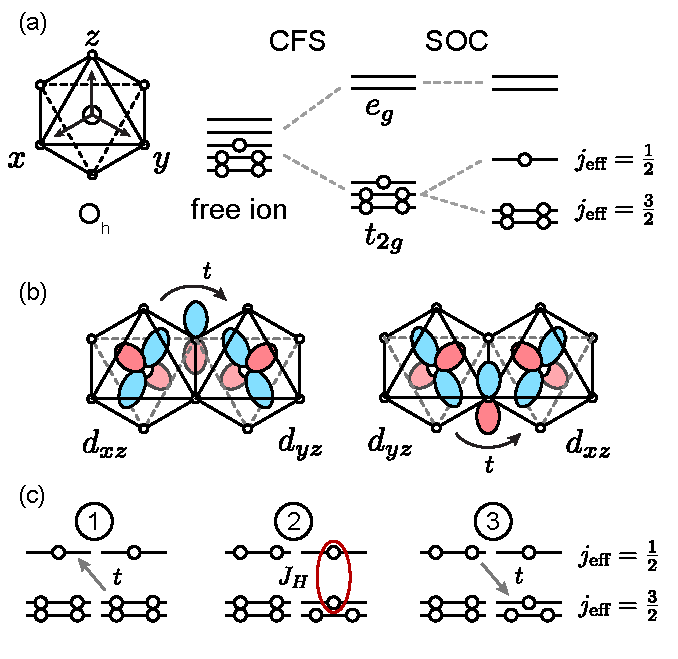
\includegraphics{images/CH3/JK-fig1.pdf}
 %  \caption{ Frontal-top view of the $\text{RuCl}_6$ octahedron with orange circle describing the Chlorine atoms and the white circle at the centre is the Ruthenium atom. The vertex of the octahedron are used to define the basis $\hat{x},\hat{y},\hat{z}$. Similar octahedron is shown in \cite{Winter_2017}.       }     \label{fig:3-Octahedron} \end{figure}

Throughout this text, I will use two cartesian bases for space.  The first basis is  $\bf{\hat{x}},\bf{\hat{y}},\bf{\hat{z}}$, and I will use this as our standard basis. The second basis is denoted by $\bf{a},\bf{b}$ and $\bf{c}$.  The vectors $\bf{a}$ and $\bf{b}$ lie in the plane of the honeycomb lattice and $\bf{c}$ is perpendicular to the plane. In terms of the standard basis, the second basis is expressed as 
\begin{align}
    \bf{a} \; &= \;% \bf{b} \times \bf{c} \; = \; 
    \frac{1}{\sqrt{6}} \, (1,1,-2) 
    \; , \\[4pt]    
    \bf{b} \; &= \;  \frac{1}{\sqrt{2}} \, (-1,1,0) \; , \\[4pt]
    \bf{c} \; &= \;  \frac{1}{\sqrt{3}} \, (1,1,1) \; .
\end{align}

\begin{figure}[h]
\centering
  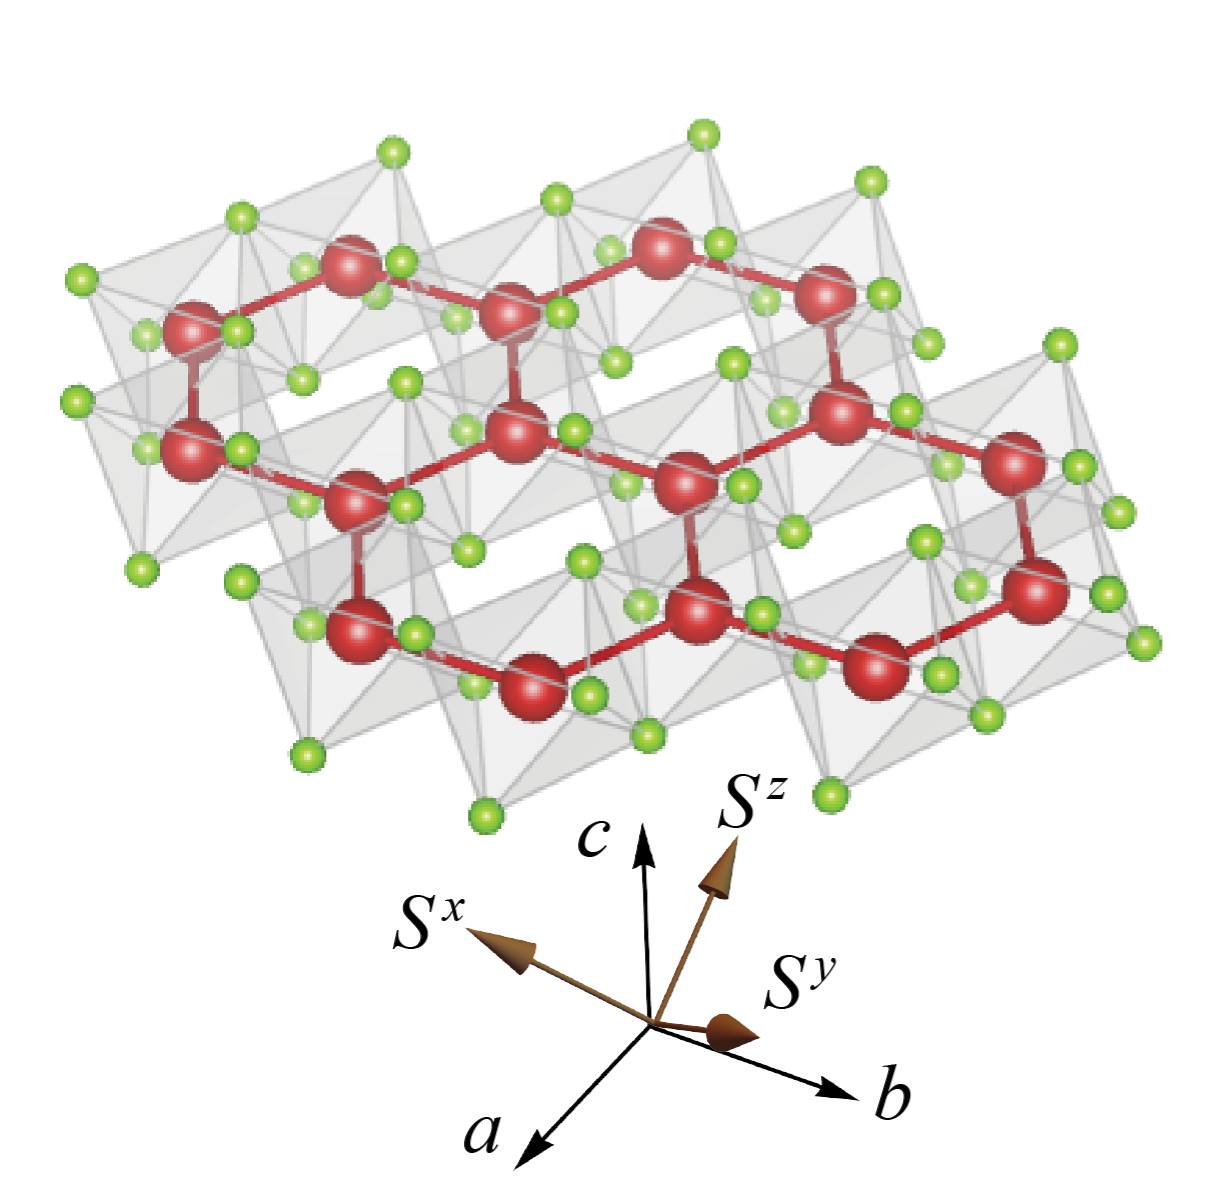
\includegraphics[width= 0.6\textwidth]{images/CH3/Fig1.png}
  \caption{ The honeycomb lattice of ruthenium atoms in red and the chlorine atoms in green. The axis $S^x,S^y, S^z$ is the basis $\bf{\hat{x}},\bf{\hat{y}},\bf{\hat{z}}$. Figure extracted from \cite{yokoi2020halfinteger}.  }
  \label{fig:3-yokoi}
  \end{figure}
  
  


%\begin{figure}[h]
%    \centering
%    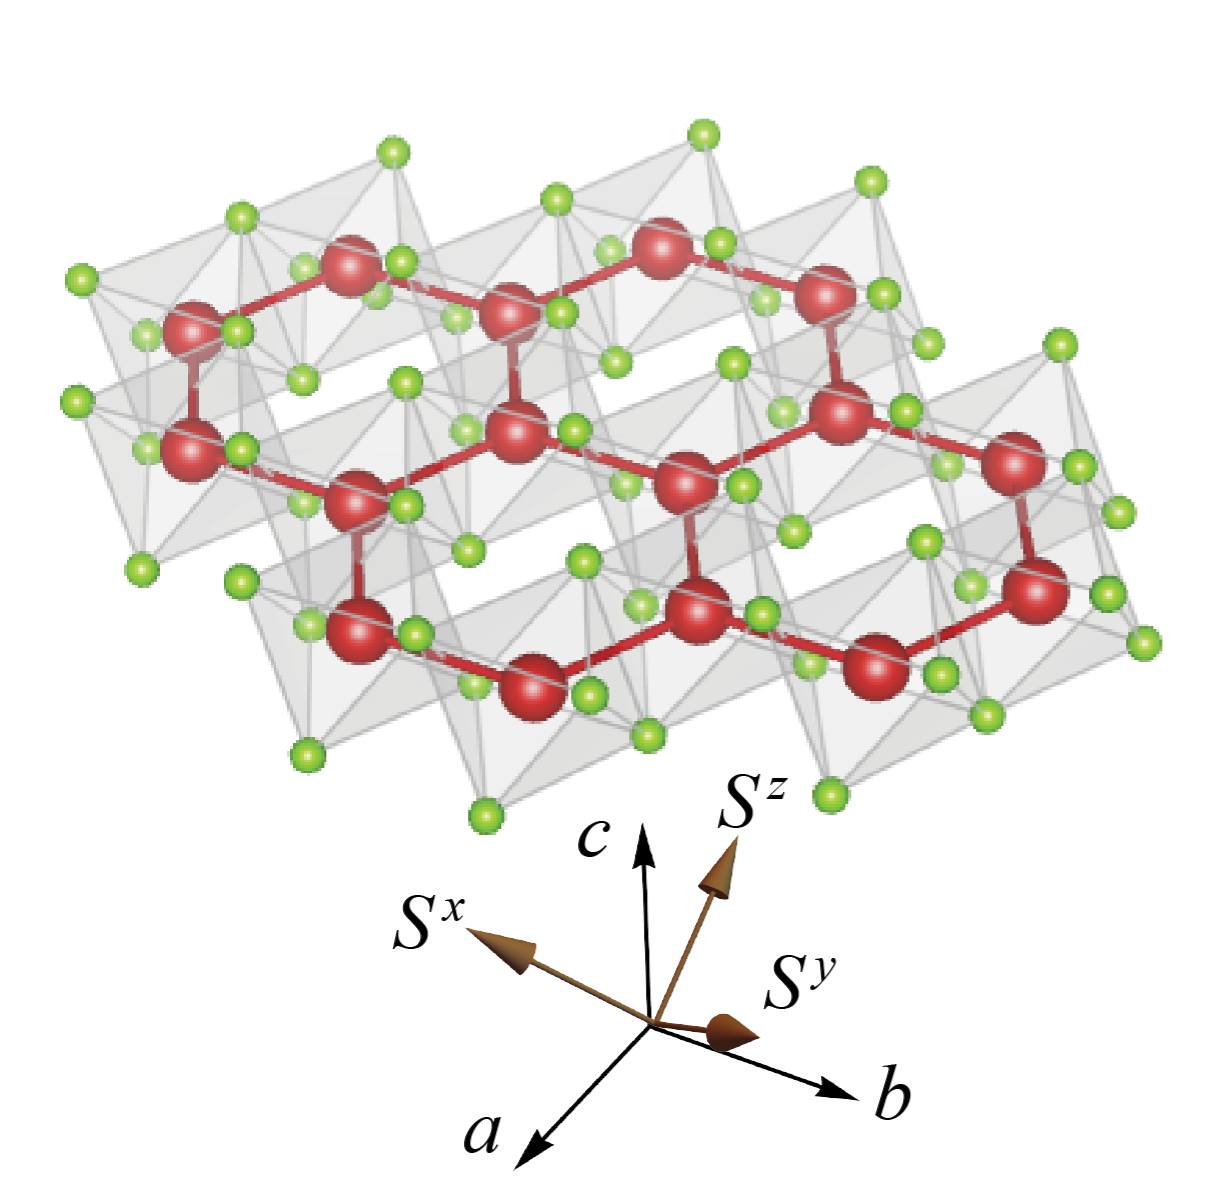
\includegraphics[width= 0.5\textwidth]{images/CH3/Fig1.png}
%    \caption{Lattice structure of \acrshort{rucl} including the Chlorine octahedron.}
%%    \label{fig:3-rucl6}
%\end{figure}

Even though $\bf{a}$ and $\bf{b}$ are always defined in the plane in the literature, their directions vary from author to author. I am following the definitions used in \cite{yokoi2020halfinteger,Liu_2018} in which $\bf{b}$ is taken to be parallel to the z-link and $\bf{a}= \bf{b} \times \bf{c} $. 

I note that the axes are respectively orthogonal to the corresponding bonds. For example, the \textit{z} type bond is in the $(1,-1,0)$ direction, while the $z$-direction is along $(0,0,1)$. If $[\gamma\text{-link}]$ denotes the unit vector in the direction of a $\gamma$ type bond, in terms of the basis these vectors are 
\begin{align}
    [x\text{-link}] \; & = \; \frac{1}{\sqrt{2}} \, \left( \, \hat{y} \; - \; \hat{z} \, \right) \; , \\
    [y\text{-link}] \; & = \; \frac{1}{\sqrt{2}} \, \left( \, \hat{z} \; - \; \hat{x} \, \right) \; , \\
    [z\text{-link}] \; & = \; \frac{1}{\sqrt{2}} \, \left( \, \hat{x} \; - \; \hat{y} \, \right) \; , 
\end{align}
see Ref.\cite{Liu_2018} for a picture of all vectors in a unit sphere.



\section{Edge modes - the microscopic Hamiltonian}

The Hamiltonian is a sum of local terms. For the terms that happen in the bulk, the Hamiltonian is the same as \eqref{2-Ham-mag}. The Hamiltonian differs at the edge, in which it is considered the Zeeman coupling $-\sum_{j} \bm{\sigma}_j \cdot \bf{h}$ without approximations. % In particular, the zigzag edge has a peculiarity that, after rewriting the spin as Majorana fermions \eqref{eq:2-maj-t}, all $b^x$ and $b^y$ are coupled into the gauge fields $u$, while $b^z$ at the edge will remain uncoupled to others $b^\alpha$ field. The dynamic of these fields appears due to the Zeeman interaction. 
The Hamiltonian is
\begin{equation}
    H \; = \; \; -  \, J \sum_{\, \langle j,k \rangle_{\alpha} }  \, \im \, \hat{u}_{jk} \, c_j c_k    \; - \; \kappa  \sum_{ \, \langle \langle i,k \rangle \rangle }   \, \im \hat{u}_{ij}\hat{u}_{jk} \,c_i c_k  \; - \; \sum_{j \in \text{Edge}} \im h_{z}b_{j}^{z} c_{j} \; . \label{eq:3-H}
\end{equation}
\begin{figure}[t]
  \begin{minipage}{.7\textwidth}
    \centering
    \scalebox{1.3}{\documentclass{standalone}  
\usepackage{tikz,comment}
\usepackage[active,tightpage]{preview}
\PreviewEnvironment{tikzpicture}
\setlength\PreviewBorder{1pt}
%%%
\usetikzlibrary{arrows} 





\begin{document}
% Define the layers to draw the diagram
\pgfdeclarelayer{background}
\pgfdeclarelayer{foreground}
\pgfsetlayers{background,main,foreground}


\def \h { 0.57735026918}  % 1/sqrt(3) comprimento  y  de uma celula                                     even (White, 2y) to odd (black ,2y+1) 
\def \d { 0.28867513459}  % 1/ 2 sqrt(3)  distancia  y  entre celulas                                   odd (black , 2y-1) to even (white , 2y)
\def \c { 0.5}           % 1/2 distancia  x  entre celulas  
\def \v { 0.86602540378 }  % sqrt(3)/ 2   distancia  y  de duas celulas                                   odd-odd or even-even 


\def \mar {0.2}  % margin for the clip

\def \l {7}         %horizontal length

\begin{tikzpicture}[>=latex]






\clip (-\mar+1-.1,  \v -2*\d -2*\d-2*\v -\mar -.5) rectangle (\l+\mar+1+.1,\v+\mar+1);

\foreach \a in {0,...,\l}{
  %      \draw[draw=blue!80!black, line width=0.40mm] ( \c +\a, \v  )-- ( \c+\a, \v + \c);
        \draw[draw=blue!80!black, line width=0.40mm] ( \c+\a, -\d )-- ( \c+\a, -\d -\v+\d);
  %      \draw[draw=blue!80!black, line width=0.40mm] ( \c +\a, \v -\c-2*\d-2*\v )-- ( \c+\a, \v -\c -\c-2*\d-2*\v);
}


\draw[<->,draw=orange!80!black, line width=0.40mm] (-\mar+1+.2,  \v+\mar+ 0.2) --  (\l+\mar+1-.7,\v+\mar+0.2);
\node at ( 3.5+.55, -\d - .15+2) [right] { \scriptsize \textcolor{orange!75!black}{\small $\ell_x$}   };

\foreach \b in {-1,0}{    
    \foreach \a in {1,3,...,\l} {
        \draw[draw=red!80!black, line width=0.40mm] ( \a , -\d +\v+ 2*\v*\b    ) -- ( \a -\c, -\d +\v+ 2*\v*\b   +\d );
        \draw[draw=green!80!black, line width=0.40mm] (\a , -\d +\v+ 2*\v*\b - \v+\d )-- ( \a -\c,  -\d +\v+ 2*\v*\b - \v);
            }   
}


\foreach \b in {-1,0}{    
    \foreach \a in {1,3,...,\l} {        
        \node[circle, fill=white, draw=black, line width=0.40mm, inner sep=2pt, minimum size=2pt] (W1\b\a) at ( \a , -\d +\v+ 2*\v*\b    ) {};
    	\node[circle, fill=black, draw=black, line width=0.40mm, inner sep=2pt, minimum size=2pt] (B2\b\a) at ( \a + \c, \v + 2*\v*\b   ) {};
        \node[circle, fill=white, draw=black, line width=0.40mm, inner sep=2pt, minimum size=2pt] (W3\b\a) at ( \a +1, -\d +\v+ 2*\v*\b    ) {};
    	\node[circle, fill=black, draw=black, line width=0.40mm, inner sep=2pt, minimum size=2pt] (B4\b\a) at ( \a +1, -\d +\v+ 2*\v*\b - \v+\d)  {};
    	\node[circle, fill=white, draw=black, line width=0.40mm, inner sep=2pt, minimum size=2pt] (W5\b\a) at ( \a -\c + 1, -\d +\v+ 2*\v*\b - \v) {};  	
    	\node[circle, fill=black, draw=black, line width=0.40mm, inner sep=2pt, minimum size=2pt] (B6\b\a) at  ( \a , -\d +\v+ 2*\v*\b - \v+\d ) {};

    	\node[circle, fill=black, draw=black, line width=0.40mm, inner sep=2pt, minimum size=2pt] (B2r\b\a) at ( \a + \c+1, -\d +\v+ 2*\v*\b+\d   ) {}; 
    	\node[circle, fill=white, draw=black, line width=0.40mm, inner sep=2pt, minimum size=2pt] (W5r\b\a) at ( \a -\c + 2, -\d +\v+ 2*\v*\b - \v) {};    	
    	
    }   
}

\foreach \b in {-1,0}{    
    \foreach \a in {1,3,...,\l} { 
        \draw[draw=green!80!black, line width=0.40mm] (B2\b\a)-- (W1\b\a);
        \draw[draw=red!80!black, line width=0.40mm] (B2\b\a)--(W3\b\a);
        \draw[draw=blue!80!black, line width=0.40mm] (W1\b\a)--(B6\b\a);
 %       \draw[draw=red!80!black, line width=0.40mm] (W1\b\a)-- ( \a -\c, -\d +\v+ 2*\v*\b   +\d );
        \draw[draw=green!80!black, line width=0.40mm] (B2r\b\a)-- (W3\b\a);        
        \draw[draw=blue!80!black, line width=0.40mm] (W3\b\a)--(B4\b\a);       
        \draw[draw=red!80!black, line width=0.40mm] (W5\b\a)--(B6\b\a);        
        \draw[draw=green!80!black, line width=0.40mm] (B4\b\a)-- (W5\b\a);
        \draw[draw=red!80!black, line width=0.40mm] (W5r\b\a)--(B4\b\a); 
%        \draw[draw=green!80!black, line width=0.40mm] (B6\b\a)-- ( \a -\c, 2*\v*\b   - \d);
            }   
}


\end{tikzpicture}
\end{document}}
    %\caption{Caption}
    %\label{fig:3-lattice}
  \end{minipage}%
  \begin{minipage}{.3\textwidth}
    \centering
    \scalebox{1.3}{\documentclass{standalone}  
\usepackage{tikz,comment}
\usepackage[active,tightpage]{preview}
\PreviewEnvironment{tikzpicture}
\setlength\PreviewBorder{1pt}
%%%
\usetikzlibrary{arrows} 





\begin{document}
% Define the layers to draw the diagram
\pgfdeclarelayer{background}
\pgfdeclarelayer{foreground}
\pgfsetlayers{background,main,foreground}


\def \h { 0.57735026918}  % 1/sqrt(3) comprimento  y  de uma celula                                     even (White, 2y) to odd (black ,2y+1) 
\def \d { 0.28867513459}  % 1/ 2 sqrt(3)  distancia  y  entre celulas                                   odd (black , 2y-1) to even (white , 2y)
\def \c { 0.5}           % 1/2 distancia  x  entre celulas  
\def \v { 0.86602540378 }  % sqrt(3)/ 2   distancia  y  de duas celulas                                   odd-odd or even-even 


\def \mar {0.2}  % margin for the clip

\def \l {7}         %horizontal length

\begin{tikzpicture}[>=latex]





\draw[<-,draw=cyan!80!black, line width=0.40mm] (2+.6, -4*\d -\v -.15 ) --  (2+.6,\v+.15);
\node at ( 2.65, -2*\d ) [right] { \scriptsize \textcolor{cyan!75!black}{\small $\ell_y$}   };
\clip (-\mar+1+ \c-.75,  \v -2*\d -2*\d-2*\v -\mar -.5) rectangle (\mar+2+.75+.3,\v+\mar+1);

\foreach \a in {1}{
  %      \draw[draw=blue!80!black, line width=0.40mm] ( \c +\a, \v  )-- ( \c+\a, \v + \c);
        \draw[draw=blue!80!black, line width=0.40mm] ( \c+\a, -\d )-- ( \c+\a, -\d -\v+\d);
  %      \draw[draw=blue!80!black, line width=0.40mm] ( \c +\a, \v -\c-2*\d-2*\v )-- ( \c+\a, \v -\c -\c-2*\d-2*\v);
}


\foreach \b in {-1,0}{    
    \foreach \a in {1} {
   %     \draw[draw=red!80!black, line width=0.40mm] ( \a , -\d +\v+ 2*\v*\b    ) -- ( \a -\c, -\d +\v+ 2*\v*\b   +\d );
  %      \draw[draw=green!80!black, line width=0.40mm] (\a , -\d +\v+ 2*\v*\b - \v+\d )-- ( \a -\c,  -\d +\v+ 2*\v*\b - \v);
            }   
}


\foreach \b in {-1,0}{    
    \foreach \a in {1} {    
    	\node[circle, fill=black, draw=black, line width=0.40mm, inner sep=2pt, minimum size=2pt] (B2\b\a) at ( \a + \c, \v + 2*\v*\b   ) {};
        \node[circle, fill=white, draw=black, line width=0.40mm, inner sep=2pt, minimum size=2pt] (W3\b\a) at ( \a +1, -\d +\v+ 2*\v*\b    ) {};
    	\node[circle, fill=black, draw=black, line width=0.40mm, inner sep=2pt, minimum size=2pt] (B4\b\a) at ( \a +1, -\d +\v+ 2*\v*\b - \v+\d)  {};
    	\node[circle, fill=white, draw=black, line width=0.40mm, inner sep=2pt, minimum size=2pt] (W5\b\a) at ( \a -\c + 1, -\d +\v+ 2*\v*\b - \v) {};  	
 %   	\node[circle, fill=black, draw=black, line width=0.40mm, inner sep=2pt, minimum size=2pt] (B6\b\a) at  ( \a , -\d +\v+ 2*\v*\b - \v+\d ) {};
    %	\node[circle, fill=black, draw=black, line width=0.40mm, inner sep=2pt, minimum size=2pt] (B2r\b\a) at ( \a + \c+1, -\d +\v+ 2*\v*\b+\d   ) {}; 
%    	\node[circle, fill=white, draw=black, line width=0.40mm, inner sep=2pt, minimum size=2pt] (W5r\b\a) at ( \a -\c + 2, -\d +\v+ 2*\v*\b - \v) {};    		
    }   
}


        \draw[draw=red!80!black, line width=0.40mm] (B201)--(W301);
  %      \draw[draw=green!80!black, line width=0.40mm] (B2r01)-- (W301);        
        \draw[draw=blue!80!black, line width=0.40mm] (W301)--(B401);       
  %      \draw[draw=red!80!black, line width=0.40mm] (W501)--(B601);        
        \draw[draw=green!80!black, line width=0.40mm] (B401)-- (W501);
        \draw[draw=red!80!black, line width=0.40mm] (B2-11)--(W3-11);
    %    \draw[draw=green!80!black, line width=0.40mm] (B2r-11)-- (W3-11);        
        \draw[draw=blue!80!black, line width=0.40mm] (W3-11)--(B4-11);       
     %   \draw[draw=red!80!black, line width=0.40mm] (W5-11)--(B6-11);        
        \draw[draw=green!80!black, line width=0.40mm] (B4-11)-- (W5-11);


\end{tikzpicture}
\end{document}}
    %\caption{Caption}
    %\label{fig:3-lattice-FT}
  \end{minipage}
  \caption{(Left) The  lattice for $\ell_x = 14$ and $\ell_y=8$; the lattice continues periodically in the $x$ direction, but it is finite in the $y$ direction. (Right) After Fourier transforming in the $x$ direction, the effective lattice becomes an open chain (1D lattice). }
  \label{fig:3-lattice}
  \end{figure}
Choosing the standard gauge \eqref{eq:2-gauge-fix} the system is then invariant by discrete translations of $\bf{n}_1-\bf{n}_2=(1,0)$. 

Let suppose that the horizontal length (in the periodic direction) of the system is finite $\ell_x$ and in the vertical direction is $\ell_y$ with both even numbers.  The schematic representation is shown in  figure \ref{fig:3-lattice}.  After Fourier transforming in the $x$ direction the Majoranas are transformed into complex fields $b_{q , y}$ and $c_{q,y}$. %which for the $c$ fermions the integer index $y$ indicates the vertical position,% and is even or odd if the Majorana fermions was defined at the lattice % while for $b$ it take two values $1$ or $\ell_y$ depending if the term is at the upper edge ($\mathcal{L}_{\text{O}}$, colour black in the figure) or at the lower edge ($\mathcal{L}_{\text{E}}$, colour white).
\begin{align}
     \tilde{A}_{y_1y_2}(q)  \; &= \;  \sum_{x} \, e^{\im qx} A_{0y_1,xy_2} \; \label{eq:3-fourier-t} , \\[6pt]
    c_{q,y} \; &= \; \frac{1}{\sqrt{2\ell_x}} \, \sum_{x} \, e^{- \im q x} c_{xy} \; ,  \label{eq:3-fourier-t-c}  \\[6pt]
    b^{z}_{q,y} \; &= \; \frac{1}{\sqrt{2\ell_x}} \, \sum_{x} \, e^{- \im q x} b^{z}_{xy} \; , \quad \text{for } y = 1 \text{ or } \ell_{y} \, .
\end{align}
The momentum is discretized in to the \acrlong{bz}: $\text{BZ}= \big\{  \frac{2\pi n}{\ell_x} \, \Big\vert \,  n = -\frac{\ell_x}{2}+1 , $ $...,\frac{\ell_x}{2} \big\}$. The normalization factors are chosen so that $c_{q,y}$ and $ b^{z}_{q,y}$ obeys the usual anticommutation relations for complex fermions when restricted to positive momentum. The restriction is called \acrfull{hbz} and it is $\frac{1}{2}\text{BZ}= \left\{  \frac{2\pi}{\ell_x}, \frac{4\pi}{\ell_x}, ,...,\pi  \right\}$. For example, with this normalization, the inverse Fourier transform for the Majorana operators is
\begin{align}
    c_{xy} \; &= \; \sqrt{\frac{2}{\ell_x}} \, \sum_{q \in \text{BZ}} \, e^{\im q x} c_{q,y}  \; = \;  \sqrt{\frac{2}{\ell_x}} \, \sum_{q \in \frac{1}{2}\text{BZ}} \, \Big( \,e^{\im q x} c_{q,y} \, + \, e^{-\im q x} c_{q,y}^{\dagger} \, \Big)\; . \label{eq:3-inverse-fourier}
\end{align}


The Hamiltonian obtained after the Fourier transform is 
\begin{equation}
    H \;= \; \sum_{q \in \frac{1}{2}\text{BZ}} \sum_{y_1,y_2 = 0}^{\ell_y+1} \, \im \tilde{A}_{y_1y_2}(q) \, c_{q,y_1}^{\dagger} c_{q,y_2}  \; ,
\end{equation}
with $c_{0} := b_1^z$, $c_{\ell_y+1} := b_{\ell_y}^z$ and $\im A$ is the  $(\ell_y+2)\times(\ell_y+2)$ Hermitean matrix
\begin{equation}
  \im \tilde{A}(q) = 
   \left(
\begin{array}{cccccccccccc}
 0 & i \gamma  & 0 & 0 & 0 & 0 & 0 & 0 & 0 & 0 %& 0 & 0 
 \\
 -i \gamma  & \alpha  & i s & \textcolor{black!60}{-\textcolor{black!60}{\beta}}  & 0 & 0 & 0 & 0 & 0 & 0% & 0 & 0 
 \\
 0 & -i s & -\alpha  & \textcolor{black!60}{i r} & \textcolor{black!60}{\beta}  & 0 & 0 & 0 & 0 & 0% & 0 & 0 
 \\
 0 & \textcolor{black!60}{-\textcolor{black!60}{\beta}}  & \textcolor{black!60}{- i r} & \alpha  & i s & \textcolor{black!60}{-\textcolor{black!60}{\beta}}  & 0 & 0 & 0 & 0% & 0 & 0
 \\
 0 & 0 & \textcolor{black!60}{\beta}  & -i s & -\alpha  & \textcolor{black!60}{i r} & \textcolor{black!60}{\beta}  & 0 & 0 & 0 %& 0 & 0
 \\
 0 & 0 & 0 & \ddots  &  \ddots & \ddots  & \ddots & \ddots  & 0 & 0% & 0 & 0
 \\
 0 & 0 & 0 & 0 & \ddots & \ddots & \ddots  & \ddots &  \ddots  & 0 & % 0 & 0 
 \\%
 %0 & 0 & 0 & 0 & 0 & \textcolor{black!60}{-\textcolor{black!60}{\beta}}  & \textcolor{black!60}{- i r} & \alpha  & i s & \textcolor{black!60}{-\textcolor{black!60}{\beta}}  & 0 & 0 \\ 
% 0 & 0 & 0 & 0 & 0 & 0 & \textcolor{black!60}{\beta}  & -i s & -\alpha  & \textcolor{black!60}{i r} & \textcolor{black!60}{\beta}  & 0 \\
% 0 & 0 &
0 & 0 & 0 & 0 & 0 & \textcolor{black!60}{-\textcolor{black!60}{\beta}}  & \textcolor{black!60}{- i r} & \alpha  & i s & 0 \\
% 0 & 0 &
0 & 0 & 0 & 0 & 0 & 0 & \textcolor{black!60}{\beta}  & -i s & -\alpha  & -i \gamma  \\
% 0 & 0 & 
0 & 0 & 0 & 0 & 0 & 0 & 0 & 0 & i \gamma  & 0 \\
\end{array}
\right) \,  , \label{eq:3-hamiltonian}
%\begin{pmatrix}    c_{k}(1) \\ c_{k}(2) \\c_{k}(3) \\c_{k}(4) \\c_{k}(5)\\ \vdots\\ \vdots \\ c_{k}(-4) \\ c_{k}(-3) \\
%    c_{k}(-2) \\    c_{k}(-1) \\    c_{k}(L) \\\end{pmatrix}
\end{equation}
in which the matrix elements are defined as 
%\begin{align}    \alpha       & = 4  \, \kappa  \, \sin(q) \, ,  \\    \beta        & = 4  \, \kappa  \, \sin(q/2) \, ,  \\    r               & = 2  J  \,  ,   \\    s               & = -4   \, J \, \cos(q/2)   \, , \quad \text{and} \\      \gamma         &   = - 2 h_{z} \;. \end{align}
\begin{align}
    \alpha       & = 2\, \kappa  \, \sin(q) \, ,  \\
    \beta        & = 2  \, \kappa  \, \sin(q/2) \, ,  \\
    r               & =   J  \,  ,   \\
    s               & = -2   \, J \, \cos(q/2)   \, , \\  
    \gamma          &   = - h_{z} \;.
\end{align}
The indices for matrix elements of $\tilde{A}(q)$ are allowed to take values between $0$ and $\ell_y+1$. The zeroth row and column are associated with the $b^z$ at $y=1$, as well as the last ($\ell_y+1$-th) row and column are associated with $b^z$ at $y=\ell_y$. With this terminology, the sites with $y=0$ or $y=\ell_y+1$ can be thought of as fictitious new two sites in which the $b$ fermions live.  

The couplings $\alpha$ and $s$ acts inside the unit cell, while $\beta$ and $r$ couples different unit cells. 
The $r$ and $s$ terms are directly understood as a representation of the \acrshort{nn} interaction in \eqref{eq:3-H}, and the $\alpha$ and $\beta$ are representations of the \acrshort{nnn}. Importantly, the $\gamma$ coupling is the Zeeman terms and is the one that couples $b^z$ and $c$ at the edge. That is, for a strong $\gamma$ these modes are hybridized. 

\section{Dispersion of the chiral models}

The spectrum depends on the direction and strength of the applied field. The dependence in the direction of the magnetic field enters on the Hamiltonian by the $\kappa$ dependence as the product of $h_x h_y h_z$. As known from the theory in the bulk, see chapter \ref{ch:2}, when $\kappa$ is zero the spectrum is gapless. For in-plane fields, this happens only in the discrete cases in which $\bf{h}$ is aligned to the bond directions.

 Here and in the following numerical calculations I set $\kappa = h_xh_yh_z$; this choice for proportionality constant $1$ is questionable, the predicted value is much smaller. Nevertheless, for this work this precision will not be relevant. In the calculation, I used a magnetic field of modulo $0.85 \text{ J}$. This value is arbitrary, I choose a high value for the magnetic field to amplify the contrast between different configurations. %Bear in mind that . %very signification gap in the dispersion calculated. % bear in mind that the magnetic field  $0.85$


The energy dispersion of the case in which the magnetic field is in-plane and along the z-link is shown in figure \ref{fig:3-disp-b}. The gapped behavior is in agreement with the experiment \cite{yokoi2020halfinteger} since the Hall conductivity is absent when the magnetic field is parallel to the $\bf{b}$ direction. The same dispersion for the Majorana fermions in the bulk is obtained for the field along the x-link and y-link, i.e. whenever $\kappa =0$.
 \begin{figure}[h]
    \centering
    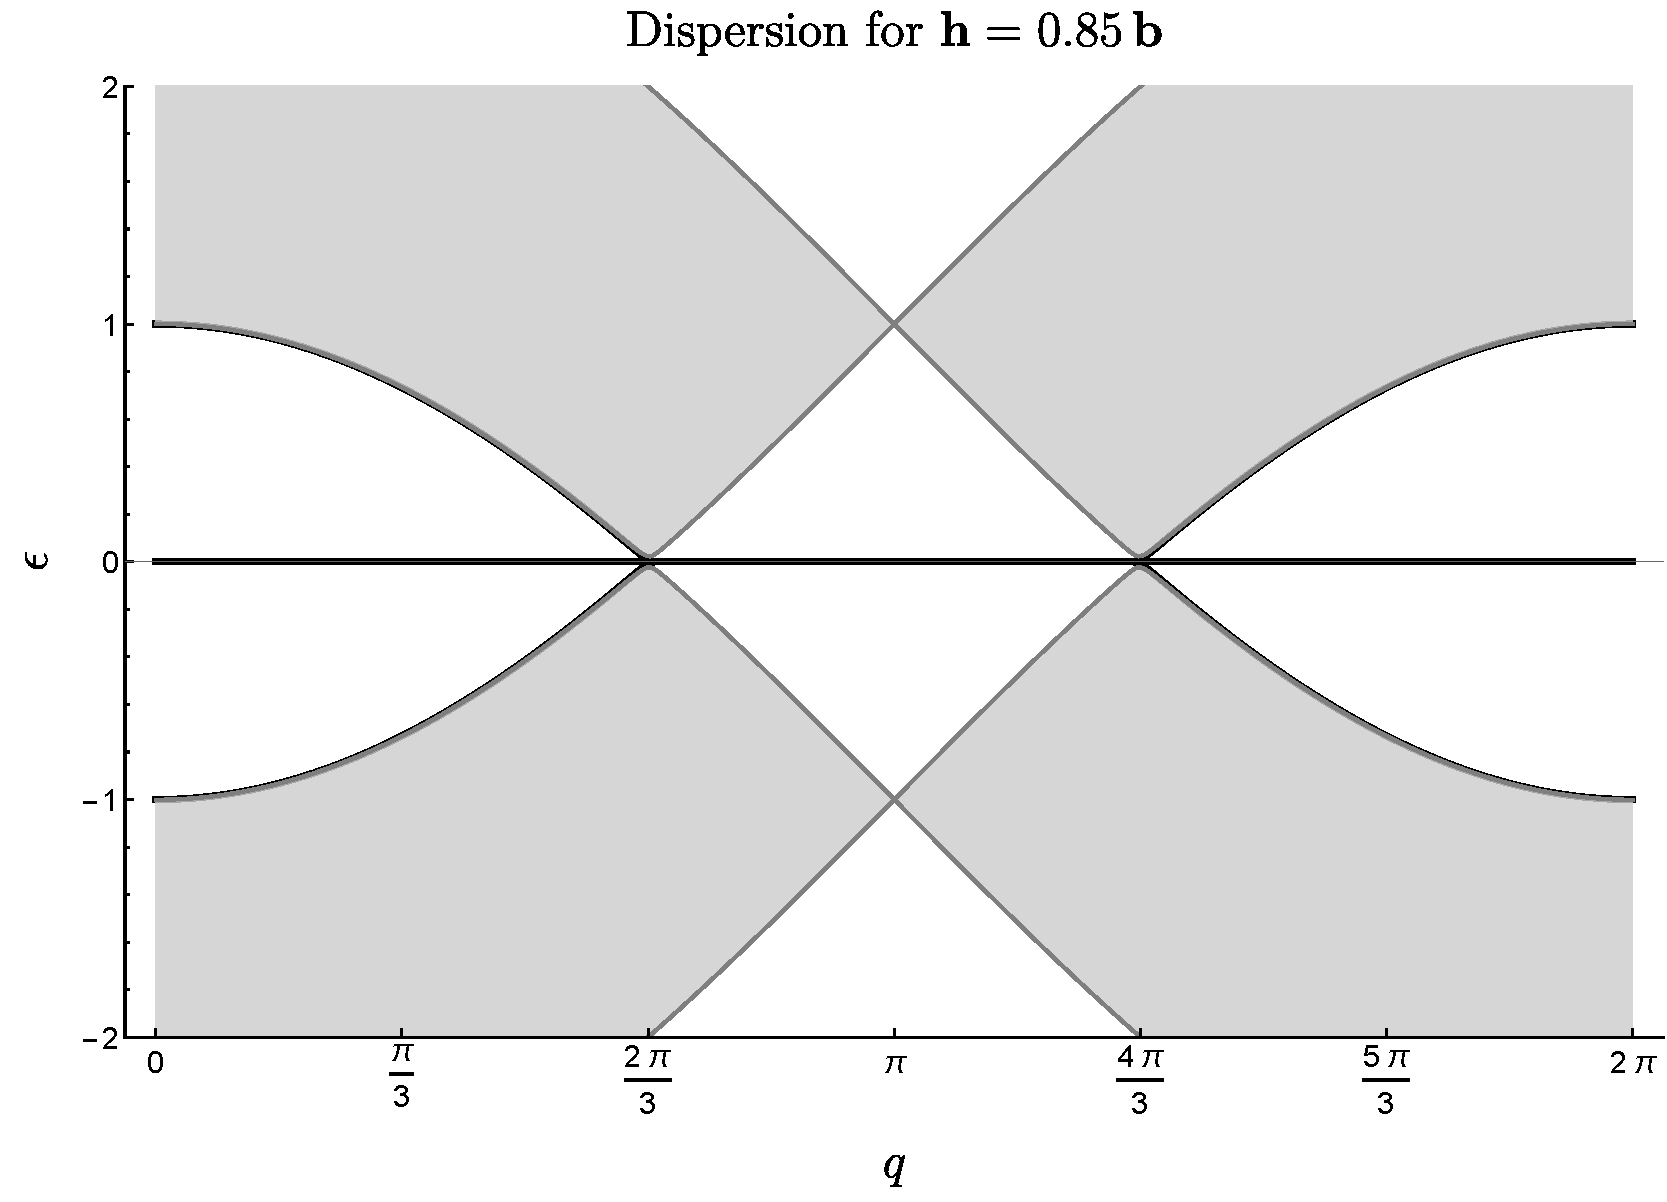
\includegraphics[width = 0.6 \textwidth]{images/CH3/disp_b.pdf}
    \caption{Magnetic field in the $\bf{b}$ direction with modulus $0.85 \, J$. The gap in the bulk is zero.  Numerical calculation was performed for $\ell_x = \ell_y = 500$, which is large enough to identify the continuum in the thermodynamic limit, and it is represented by the shaded regions. }
    \label{fig:3-disp-b}
\end{figure}
However, the edge modes obtain a non-vanishing dispersion, see figure \ref{fig:3-disp-x}, between $\frac{2\pi}{3} < q < \frac{4\pi}{3}$ for the fields in along the x- or y-link since the  $z$ component of the magnetic field is non-zero in this situation. Nonetheless, the cases in which the magnetic field point in the direction of the bond are rather exceptional cases. The generic configuration happens for $\kappa \neq 0$ and $h^z \neq 0$.

\begin{figure}[t]
    \centering
    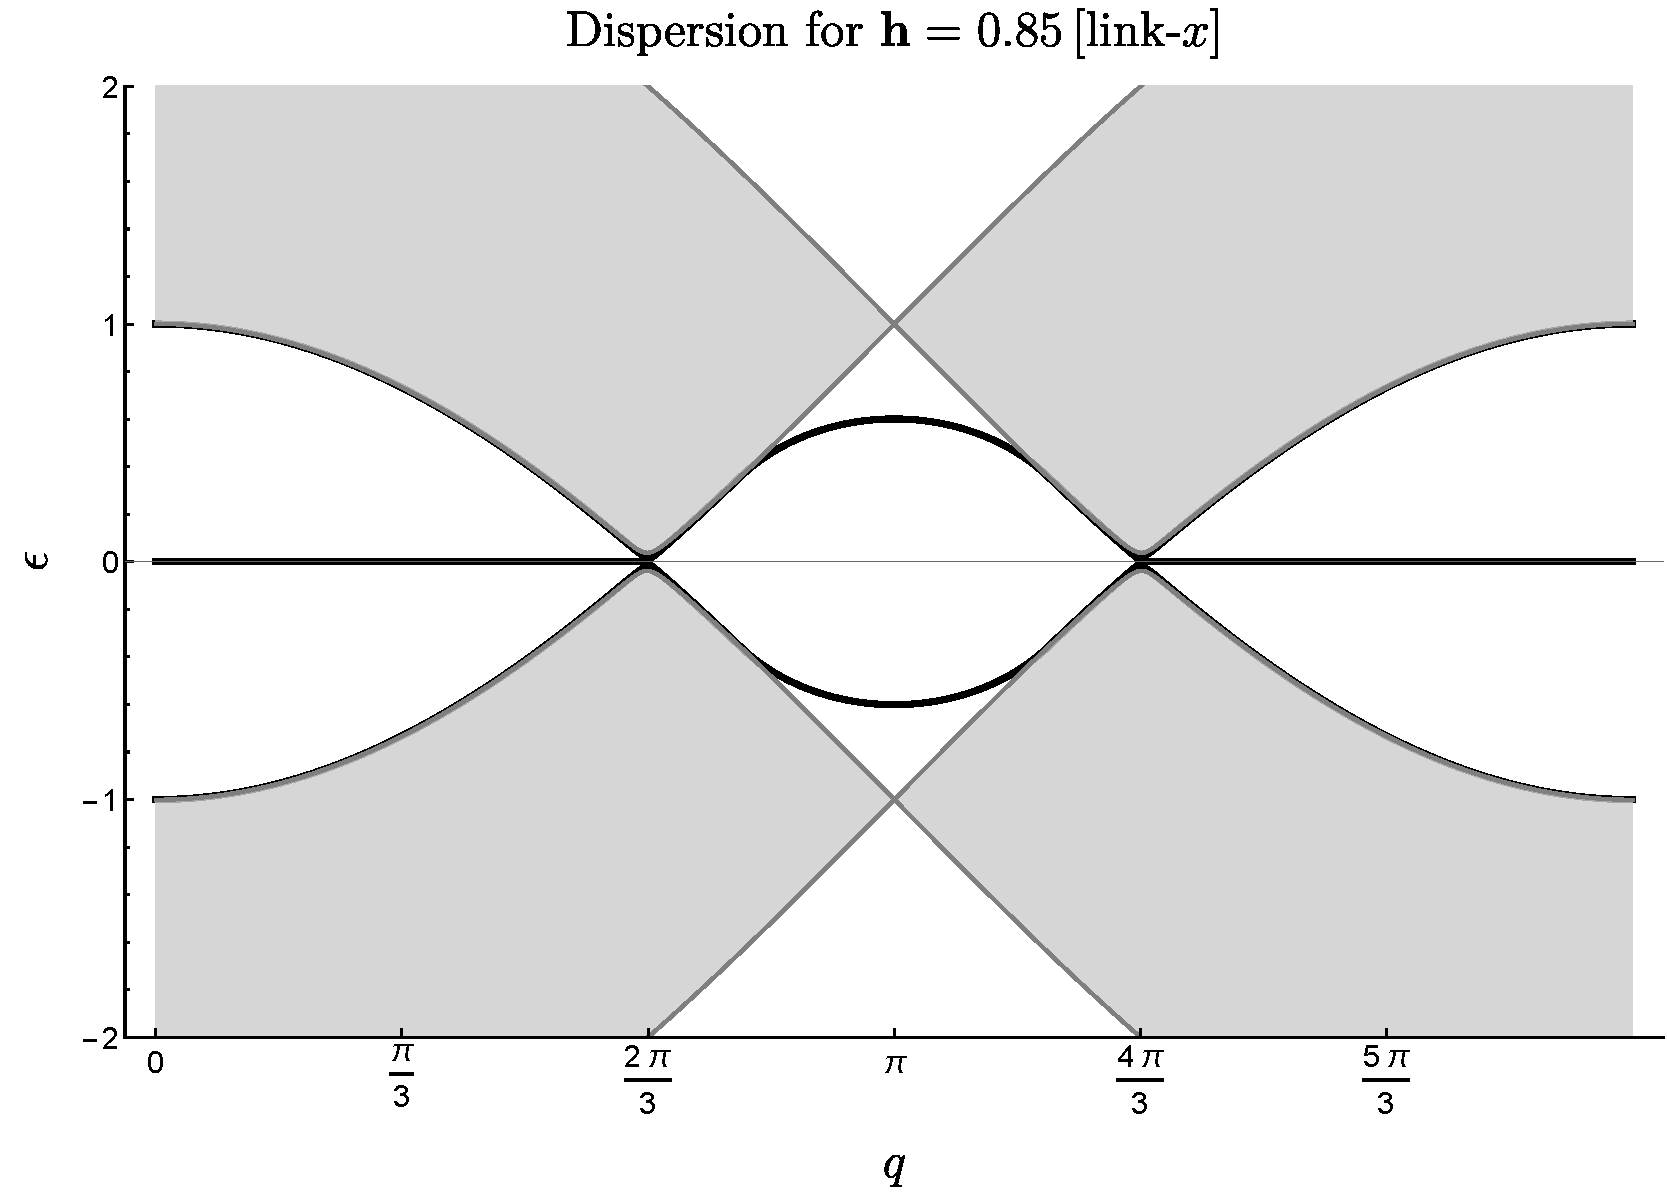
\includegraphics[width = 0.6 \textwidth]{images/CH3/disp_x.pdf}
    \caption{Magnetic field out of the plane in the $[x\text{-link}]$ direction.  }
    \label{fig:3-disp-x}
\end{figure}

Changing the direction of the magnetic field away from the bond direction make the bulk modes gapped out. The edge modes continue being gapless, but the Dirac point changes from $q=\frac{2 \pi}{3}$ to $q=0$. This gapped configuration can be seen in figures \ref{fig:3-disp-a} and \ref{fig:3-disp-c}. These two energy dispersions are qualitatively similar but differ in the magnitude of the Majorana gap.

 \begin{figure}[h]
    \centering
        \begin{subfigure}{.5\textwidth}
        \centering
        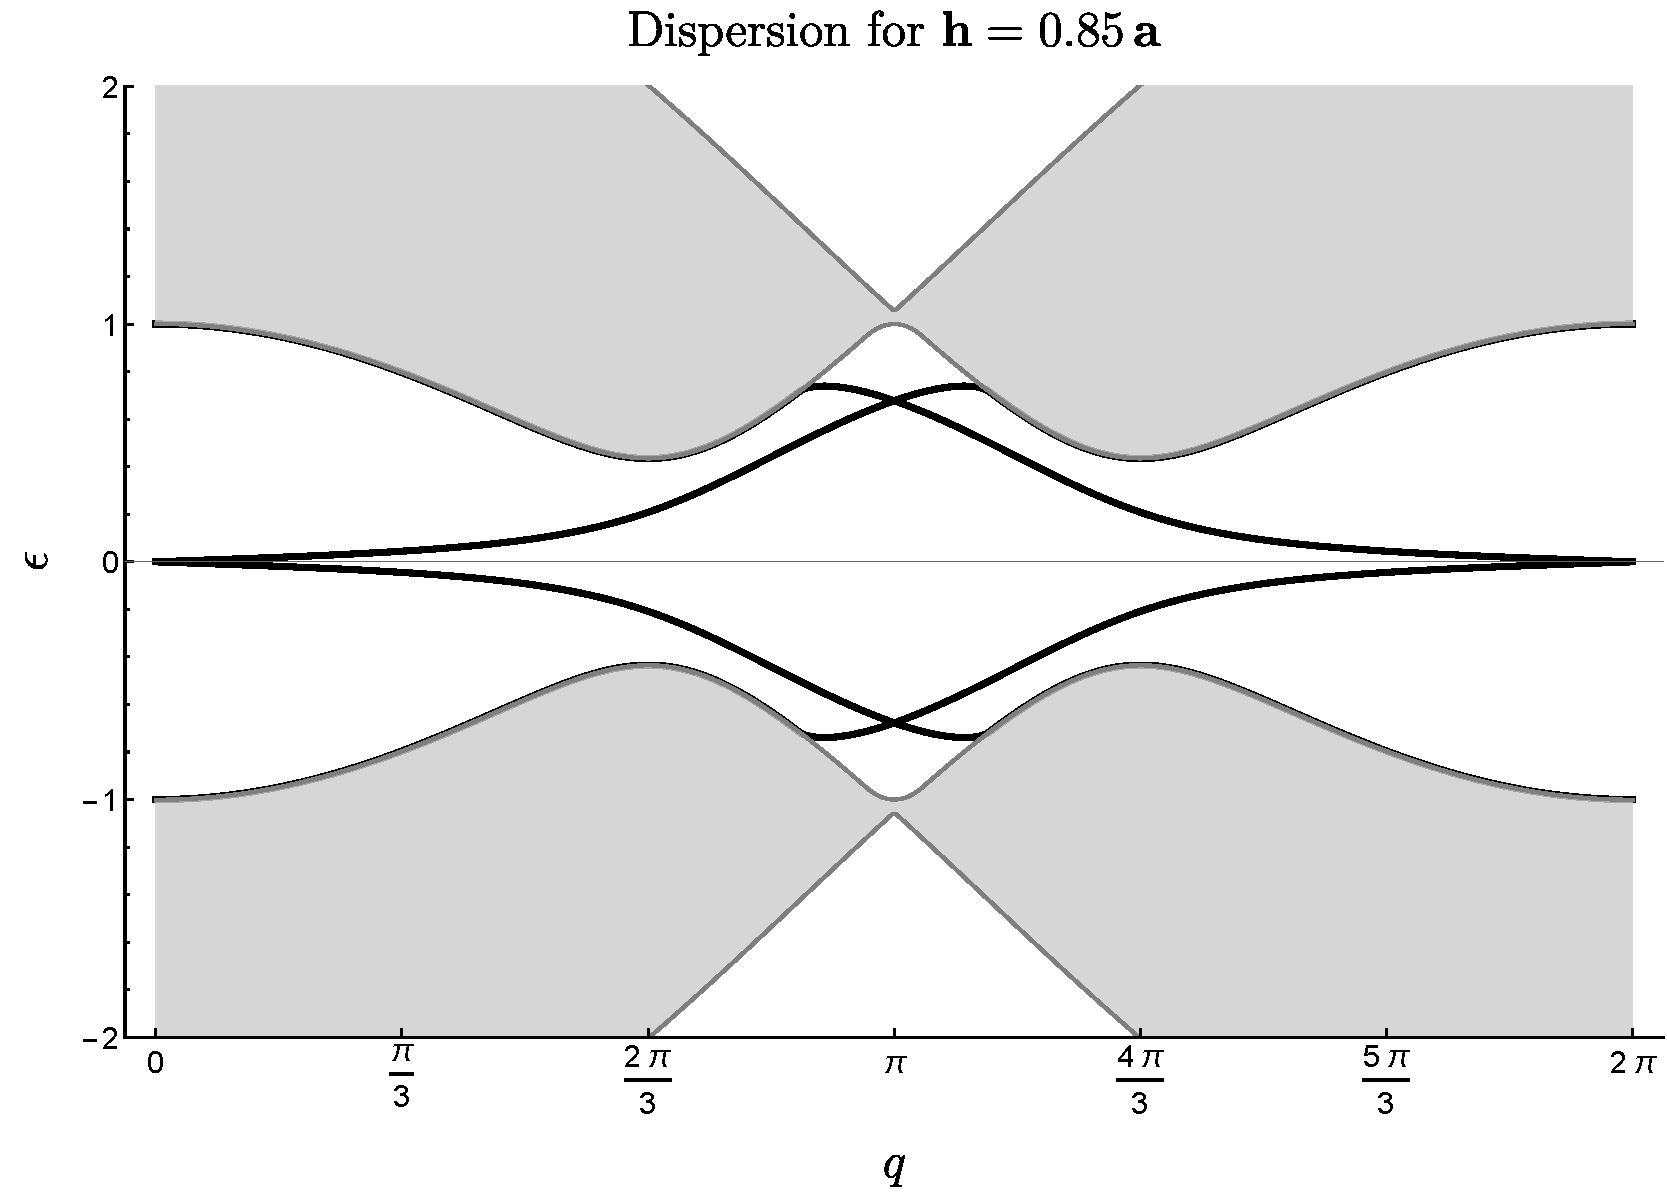
\includegraphics[width= 1.1\textwidth]{images/CH3/disp_a.pdf}
        \caption{ Magnetic field in the $\bf{a}$ direction.}
        \label{fig:3-disp-a}
    \end{subfigure}%
    \begin{subfigure}{.5\textwidth}
        \centering
        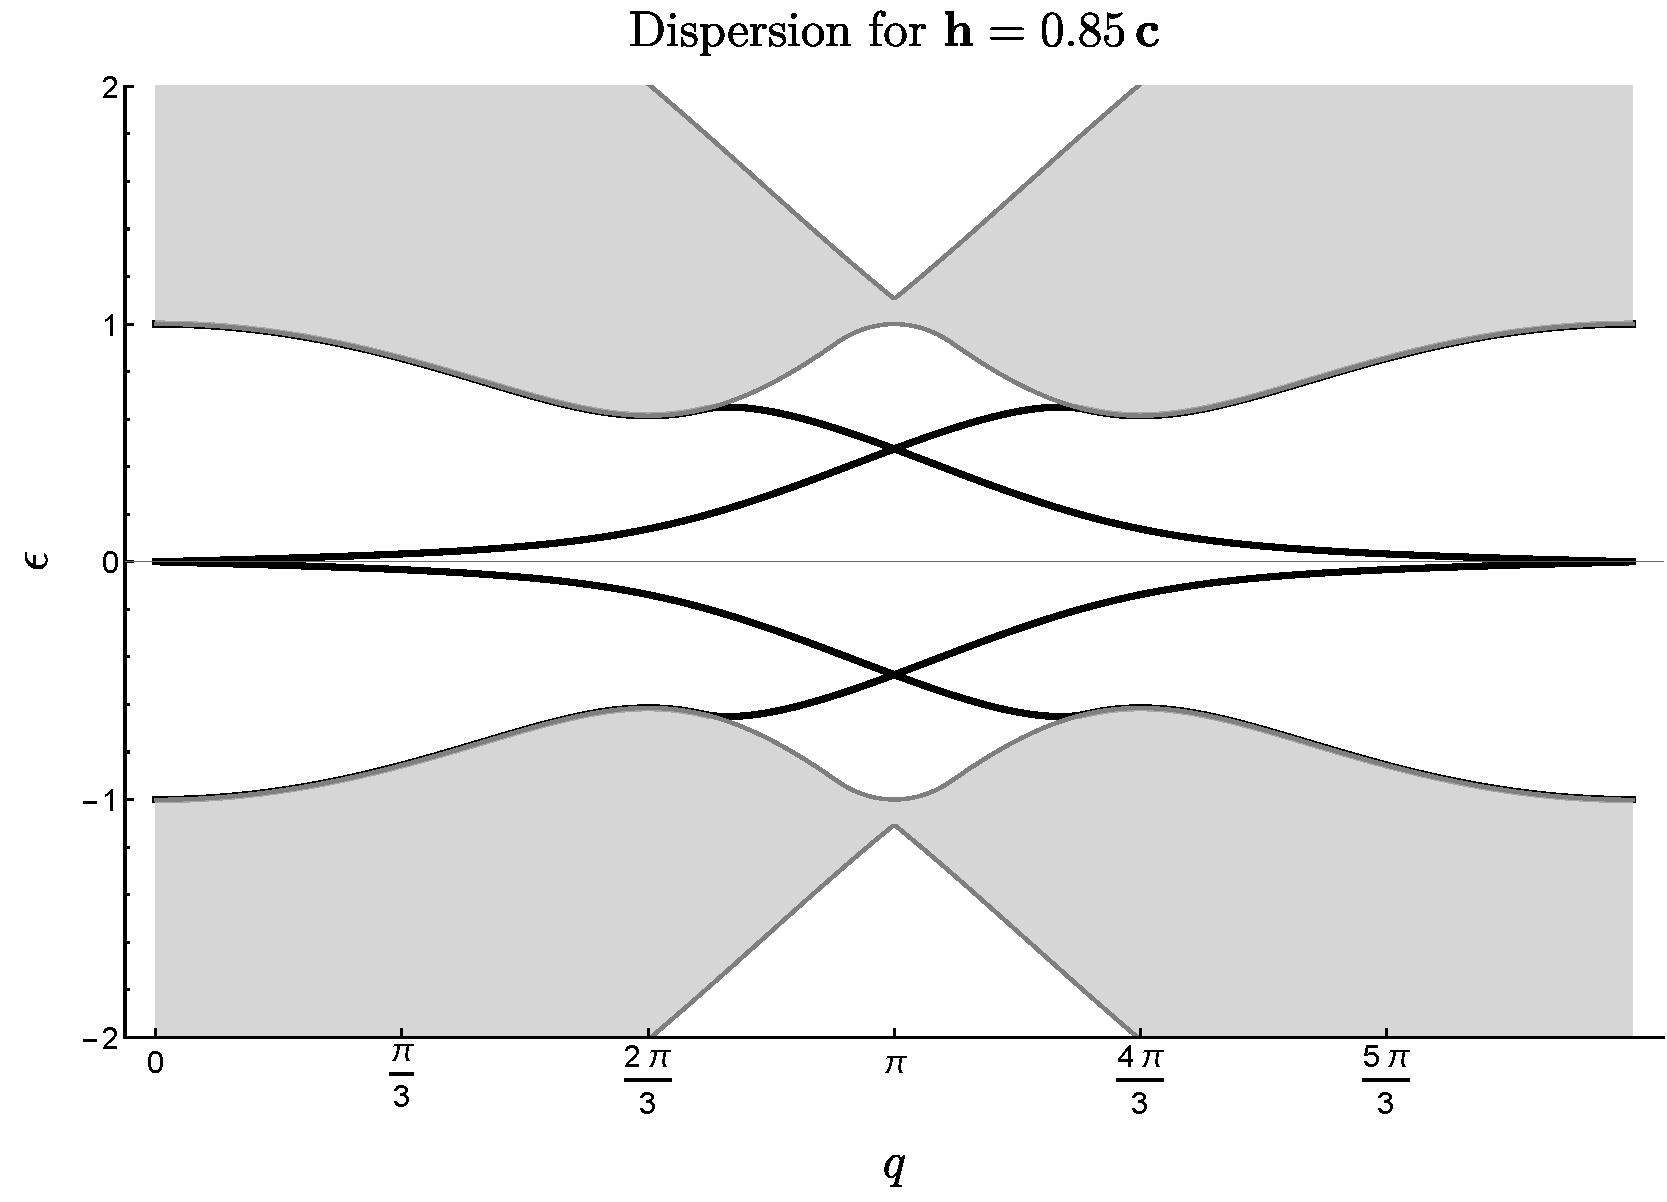
\includegraphics[width= 1.1\textwidth]{images/CH3/disp_c.pdf} 
        \caption{Magnetic field in the $\bf{c}$ direction. }
        \label{fig:3-disp-c}
    \end{subfigure}
\caption{The  Majorana fermions in the bulk are gapped, while the Majoranas modes localized at the edge are gapless. The gray area indicates the bulk spectrum, while the bold black line is for the gapless edge modes. %Dispersion for field in plane in two distinct directions.Numerical calculation for $\ell_x = \ell_y = 500$ 
}
\end{figure} 

%\begin{figure}[hb!]    \centering    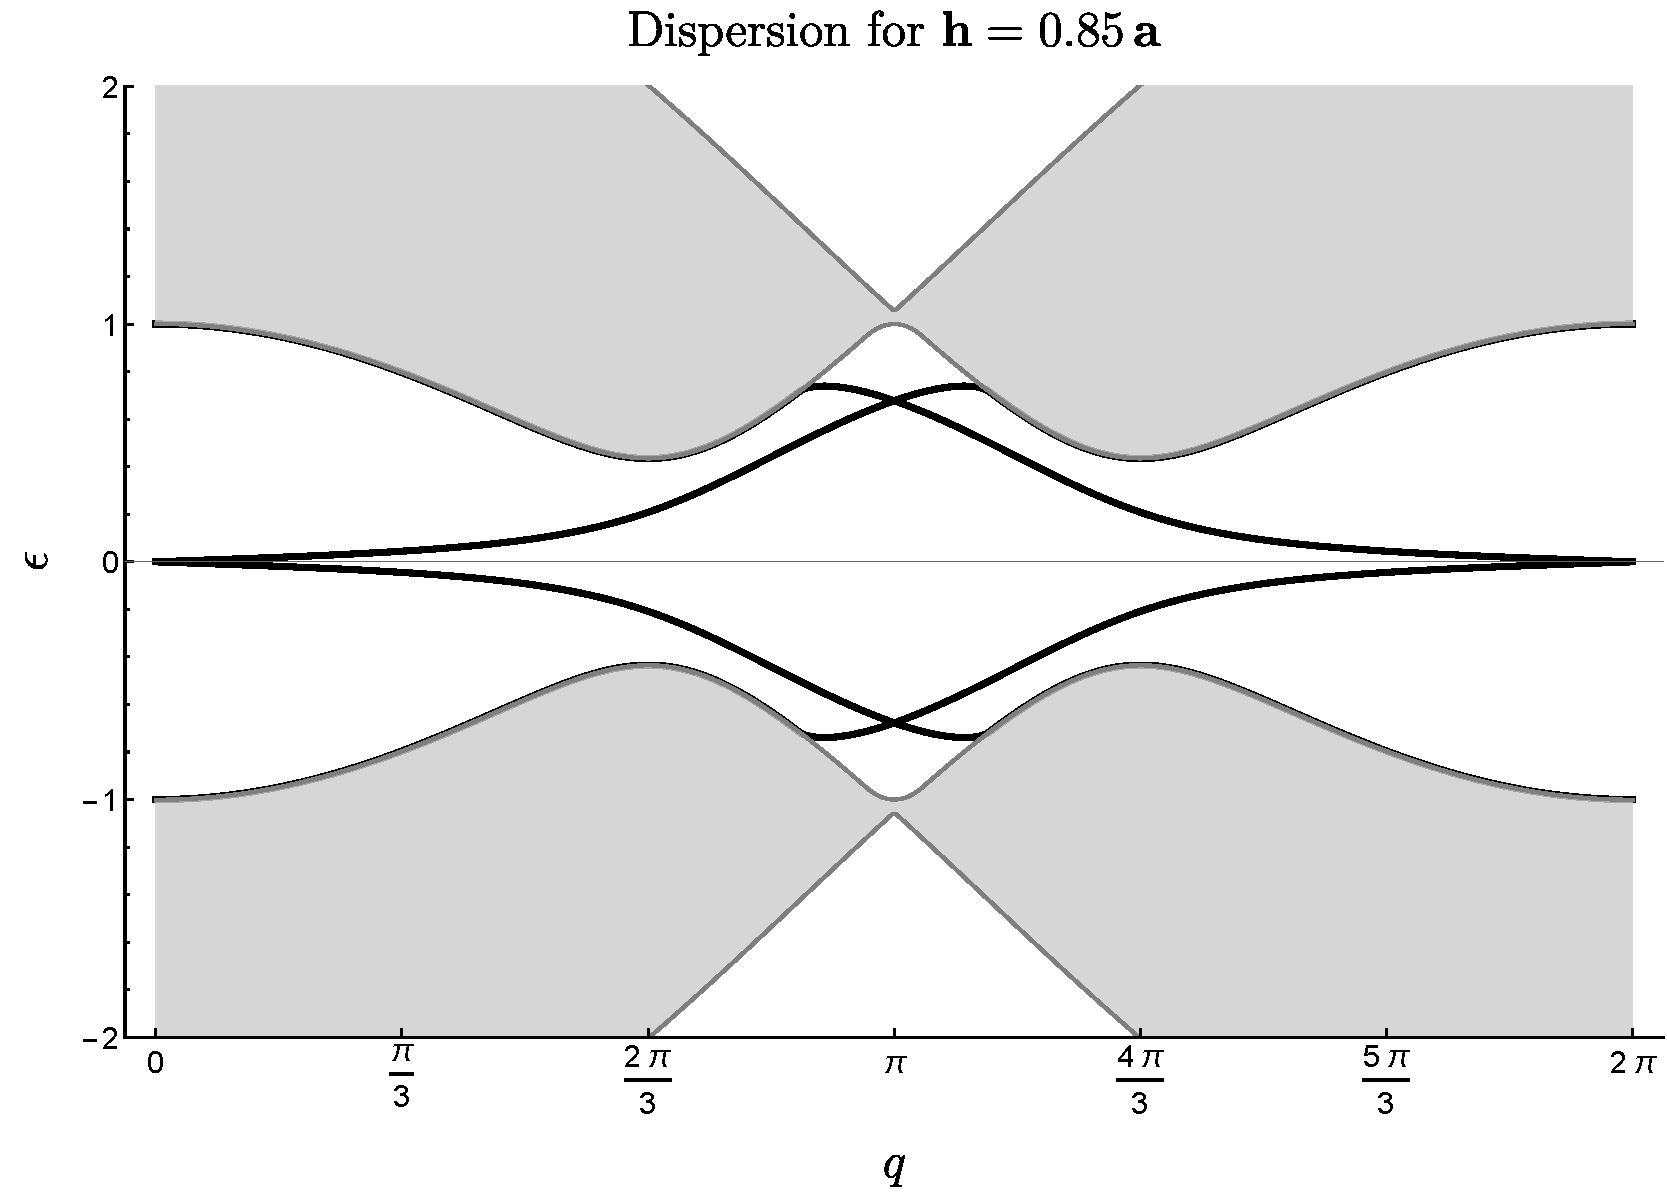
\includegraphics[width = 0.65 \textwidth]{images/CH3/disp_a.pdf}    \caption{Magnetic field in the $\bf{a}$ direction with modulus $0.85 \, J$. The bulk is gapped and the edge is gapless. The grey area indicate the bulk spectrum, while the bold black line is the gapless edge modes. }     \label{fig:3-disp-a} \end{figure}









The conclusion is that, as the direction of the magnetic field changes, the value for the gap oscillates going through zero along the lines where $h_xh_yh_z=0$ and increases in some monotonic way with the absolute value of $h_xh_yh_z$. This result is in complete agreement with the experiments \cite{yokoi2020halfinteger, tanaka2020}.


The sign of $h_xh_yh_z$, $\text{sgn}(h_xh_yh_z)$, for field $\bf{h}$ merely determines if the edge mode has positive or negative chirality, and the spectrum is equivalent. % From the figure cannot be seen but can be shown that the chiral edge modes have opposite chirality to the ones in the figures  \ref{fig:3-disp-a}  and \ref{fig:3-disp-c}, which cannot conclude just with the figure. 
As long as the magnetic field does not cross the lines where $h_xh_yh_z=0$, all octants in the $h$ space are equivalent.  %Lets consider the magnetic field in the first octant of the $h_xh_yh_z$-space. That is, consider that $h_x,h_y,h_z \geq 0$.

This calculation shows that the edge modes have linear dispersion in low energies, which allow me to define the two modes as left- and right-movers around $q=0$.  The velocity for these modes will be calculated in chapter \ref{ch:5}.

In this chapter, I established the theory that will be the base for the following chapters. Here, I have computed the microscopic Hamiltonian for a pure \acrshort{kqsl} in a geometry periodic in one direction and open in the other. In the next chapter, I will consider further interactions on this theory.



%\begin{figure}[b]% \centering     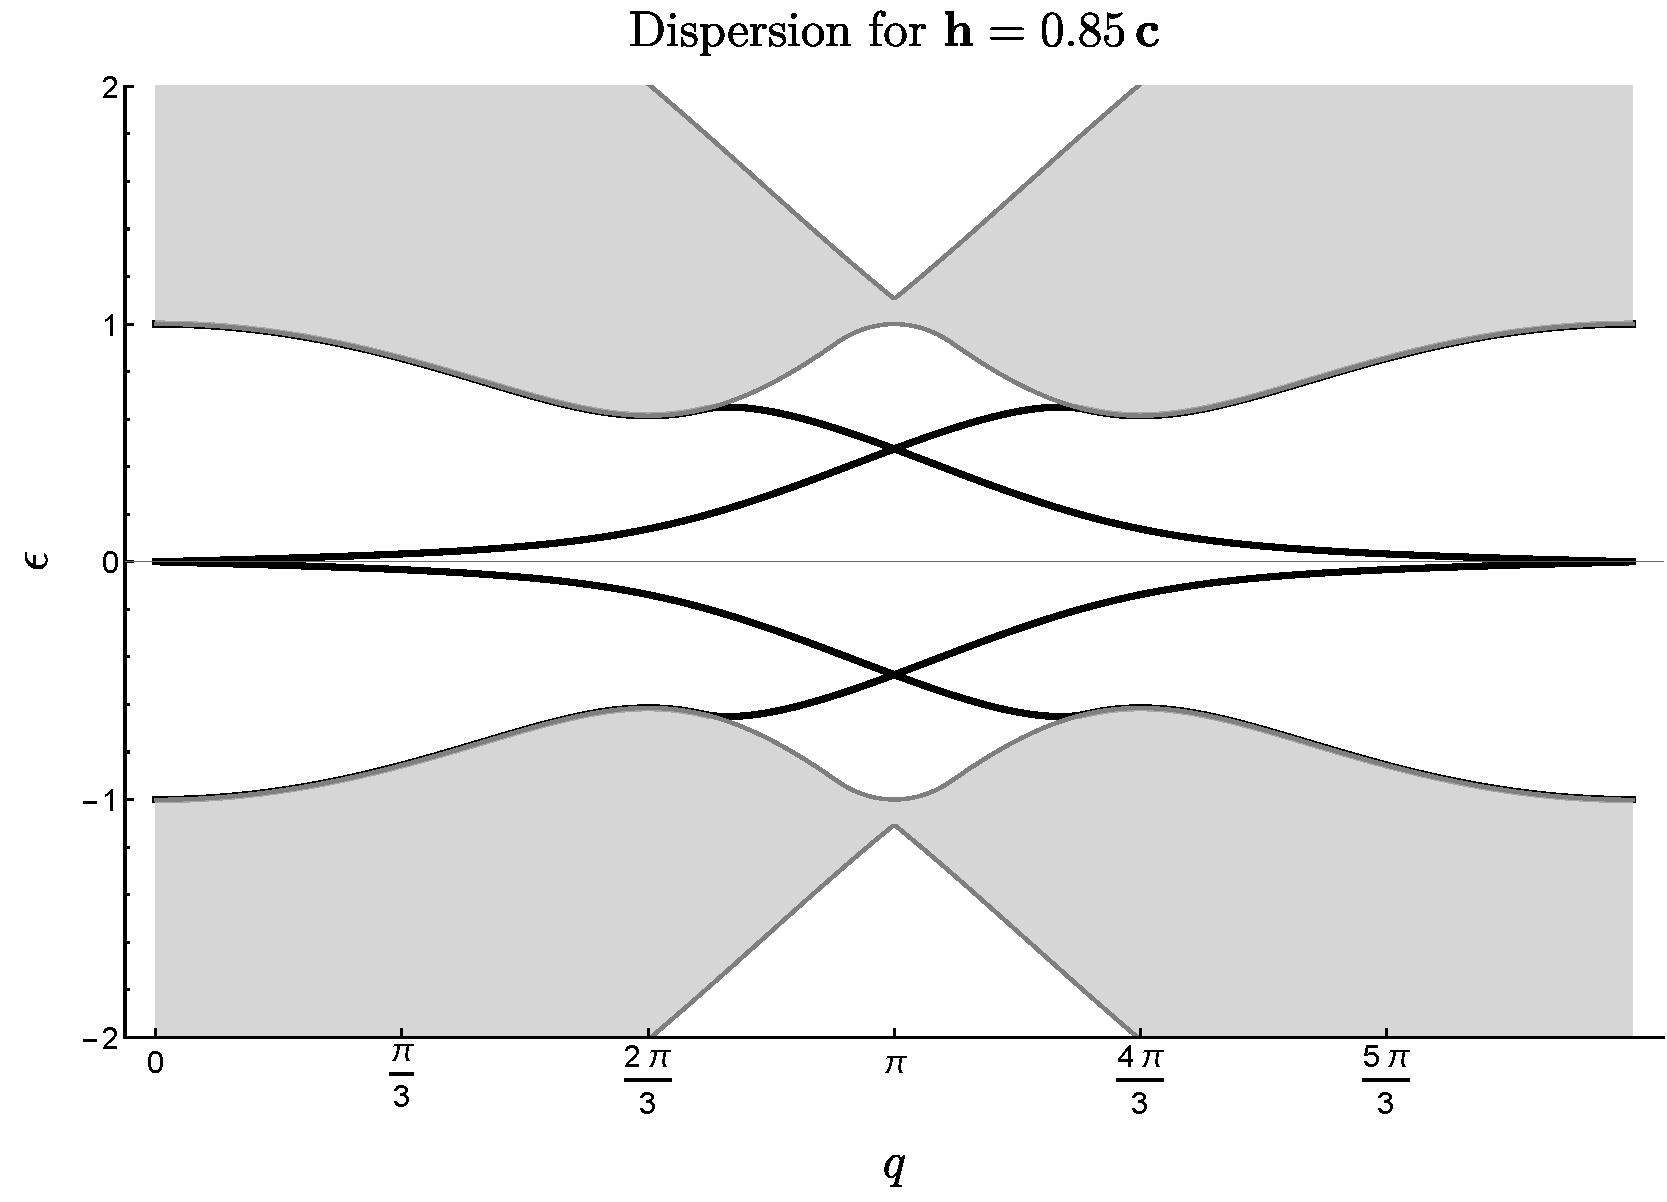
\includegraphics[width = 0.65 \textwidth]{images/CH3/disp_c.pdf}     \caption{Magnetic field out of the plane in the $\bf{c}$ direction.  }     \label{fig:3-disp-c} \end{figure}
%\begin{figure}[h]
%  \begin{minipage}{.5\textwidth}
%    \centering
%%% \end{minipage}%
  %\begin{minipage}{.5\textwidth}
  %  \centering
  %  \scalebox{1.3}{\documentclass{standalone}  
\usepackage{tikz,comment}
\usepackage[active,tightpage]{preview}
\PreviewEnvironment{tikzpicture}
\setlength\PreviewBorder{1pt}
%%%
\usetikzlibrary{arrows} 





\begin{document}
% Define the layers to draw the diagram
\pgfdeclarelayer{background}
\pgfdeclarelayer{foreground}
\pgfsetlayers{background,main,foreground}


\def \h { 0.57735026918}  % 1/sqrt(3) comprimento  y  de uma celula                                     even (White, 2y) to odd (black ,2y+1) 
\def \d { 0.28867513459}  % 1/ 2 sqrt(3)  distancia  y  entre celulas                                   odd (black , 2y-1) to even (white , 2y)
\def \c { 0.5}           % 1/2 distancia  x  entre celulas  
\def \v { 0.86602540378 }  % sqrt(3)/ 2   distancia  y  de duas celulas                                   odd-odd or even-even 


\def \mar {0.2}  % margin for the clip

\def \l {7}         %horizontal length

\begin{tikzpicture}[>=latex]





\draw[<-,draw=cyan!80!black, line width=0.40mm] (2+.6, -4*\d -\v -.15 ) --  (2+.6,\v+.15);
\node at ( 2.65, -2*\d ) [right] { \scriptsize \textcolor{cyan!75!black}{\small $\ell_y$}   };
\clip (-\mar+1+ \c-.75,  \v -2*\d -2*\d-2*\v -\mar -.5) rectangle (\mar+2+.75+.3,\v+\mar+1);

\foreach \a in {1}{
  %      \draw[draw=blue!80!black, line width=0.40mm] ( \c +\a, \v  )-- ( \c+\a, \v + \c);
        \draw[draw=blue!80!black, line width=0.40mm] ( \c+\a, -\d )-- ( \c+\a, -\d -\v+\d);
  %      \draw[draw=blue!80!black, line width=0.40mm] ( \c +\a, \v -\c-2*\d-2*\v )-- ( \c+\a, \v -\c -\c-2*\d-2*\v);
}


\foreach \b in {-1,0}{    
    \foreach \a in {1} {
   %     \draw[draw=red!80!black, line width=0.40mm] ( \a , -\d +\v+ 2*\v*\b    ) -- ( \a -\c, -\d +\v+ 2*\v*\b   +\d );
  %      \draw[draw=green!80!black, line width=0.40mm] (\a , -\d +\v+ 2*\v*\b - \v+\d )-- ( \a -\c,  -\d +\v+ 2*\v*\b - \v);
            }   
}


\foreach \b in {-1,0}{    
    \foreach \a in {1} {    
    	\node[circle, fill=black, draw=black, line width=0.40mm, inner sep=2pt, minimum size=2pt] (B2\b\a) at ( \a + \c, \v + 2*\v*\b   ) {};
        \node[circle, fill=white, draw=black, line width=0.40mm, inner sep=2pt, minimum size=2pt] (W3\b\a) at ( \a +1, -\d +\v+ 2*\v*\b    ) {};
    	\node[circle, fill=black, draw=black, line width=0.40mm, inner sep=2pt, minimum size=2pt] (B4\b\a) at ( \a +1, -\d +\v+ 2*\v*\b - \v+\d)  {};
    	\node[circle, fill=white, draw=black, line width=0.40mm, inner sep=2pt, minimum size=2pt] (W5\b\a) at ( \a -\c + 1, -\d +\v+ 2*\v*\b - \v) {};  	
 %   	\node[circle, fill=black, draw=black, line width=0.40mm, inner sep=2pt, minimum size=2pt] (B6\b\a) at  ( \a , -\d +\v+ 2*\v*\b - \v+\d ) {};
    %	\node[circle, fill=black, draw=black, line width=0.40mm, inner sep=2pt, minimum size=2pt] (B2r\b\a) at ( \a + \c+1, -\d +\v+ 2*\v*\b+\d   ) {}; 
%    	\node[circle, fill=white, draw=black, line width=0.40mm, inner sep=2pt, minimum size=2pt] (W5r\b\a) at ( \a -\c + 2, -\d +\v+ 2*\v*\b - \v) {};    		
    }   
}


        \draw[draw=red!80!black, line width=0.40mm] (B201)--(W301);
  %      \draw[draw=green!80!black, line width=0.40mm] (B2r01)-- (W301);        
        \draw[draw=blue!80!black, line width=0.40mm] (W301)--(B401);       
  %      \draw[draw=red!80!black, line width=0.40mm] (W501)--(B601);        
        \draw[draw=green!80!black, line width=0.40mm] (B401)-- (W501);
        \draw[draw=red!80!black, line width=0.40mm] (B2-11)--(W3-11);
    %    \draw[draw=green!80!black, line width=0.40mm] (B2r-11)-- (W3-11);        
        \draw[draw=blue!80!black, line width=0.40mm] (W3-11)--(B4-11);       
     %   \draw[draw=red!80!black, line width=0.40mm] (W5-11)--(B6-11);        
        \draw[draw=green!80!black, line width=0.40mm] (B4-11)-- (W5-11);


\end{tikzpicture}
\end{document}}
  %\end{minipage}
  %\caption{}
  %\label{fig:3-lattice}
  %\end{figure}
  
  
  
% \begin{figure}[h]    \begin{minipage}{.5\textwidth}     \centering       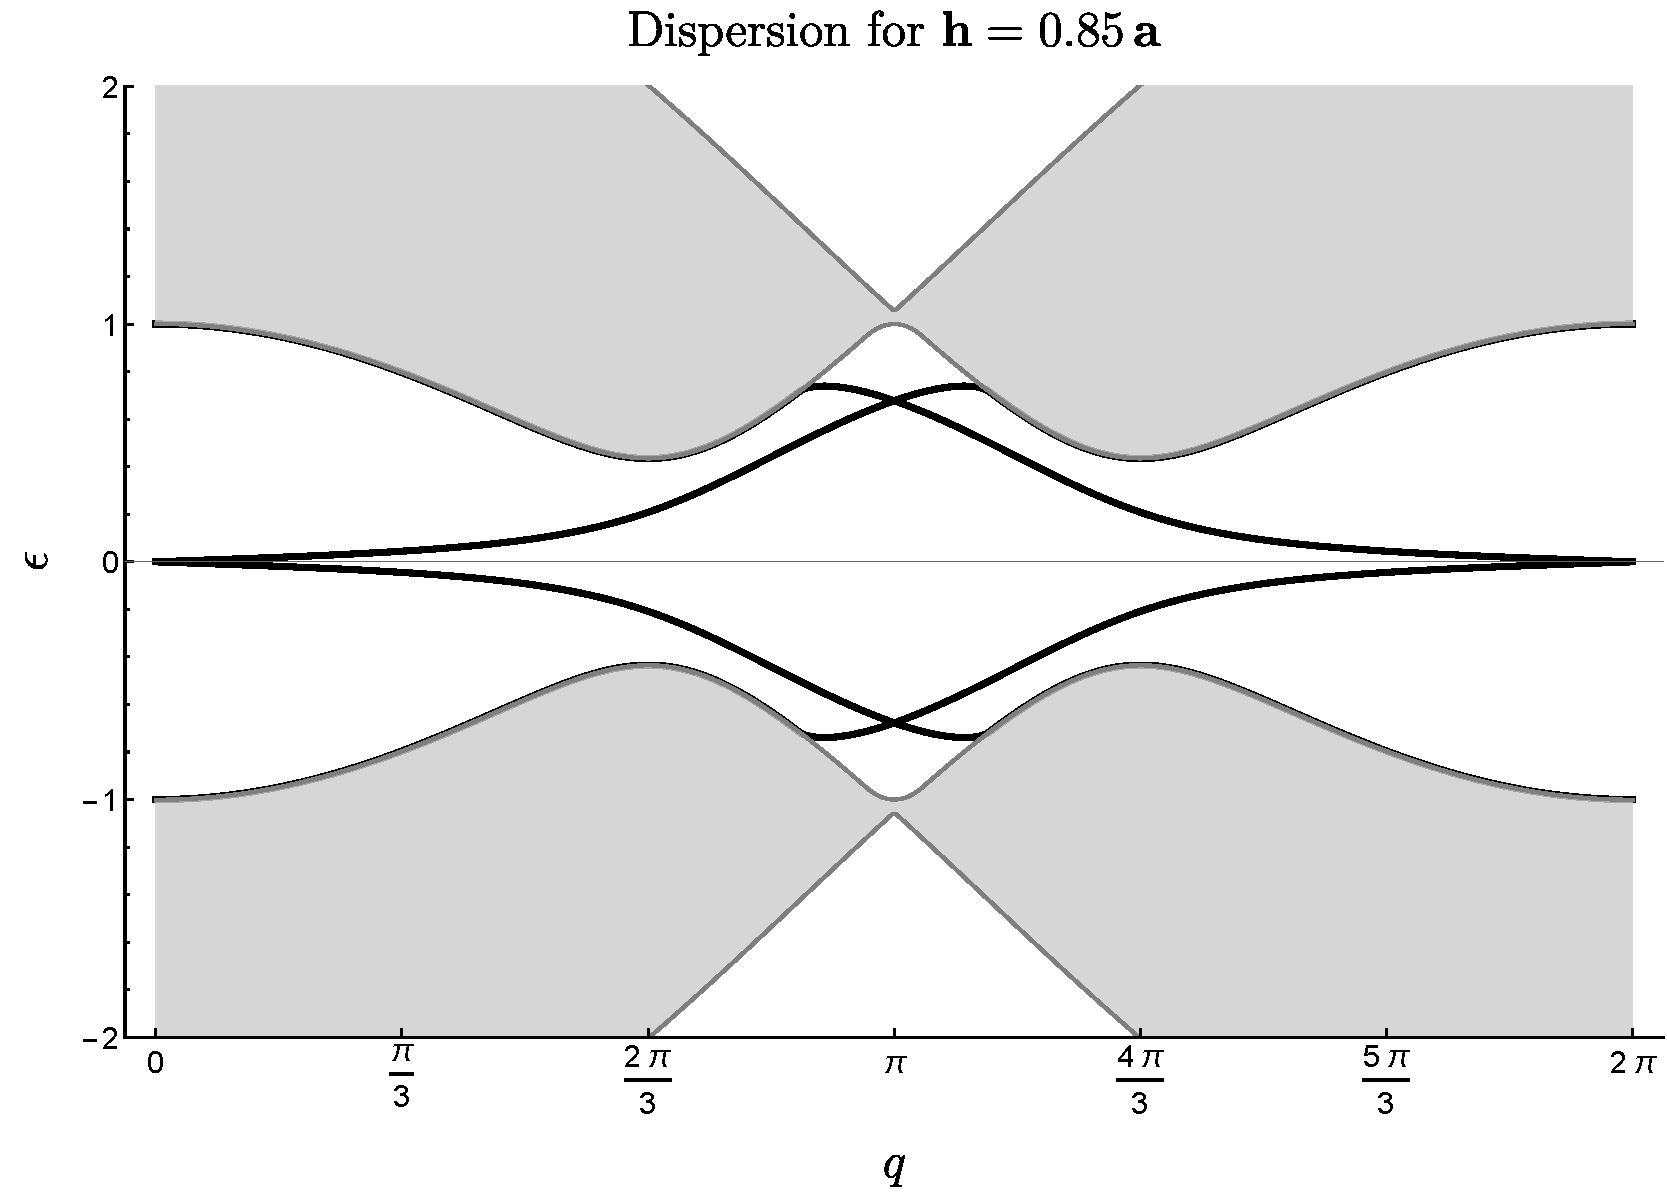
\includegraphics[width = 0.9 \textwidth]{images/CH3/disp_a.pdf}  \end{minipage}%  \begin{minipage}{.5\textwidth} \centering   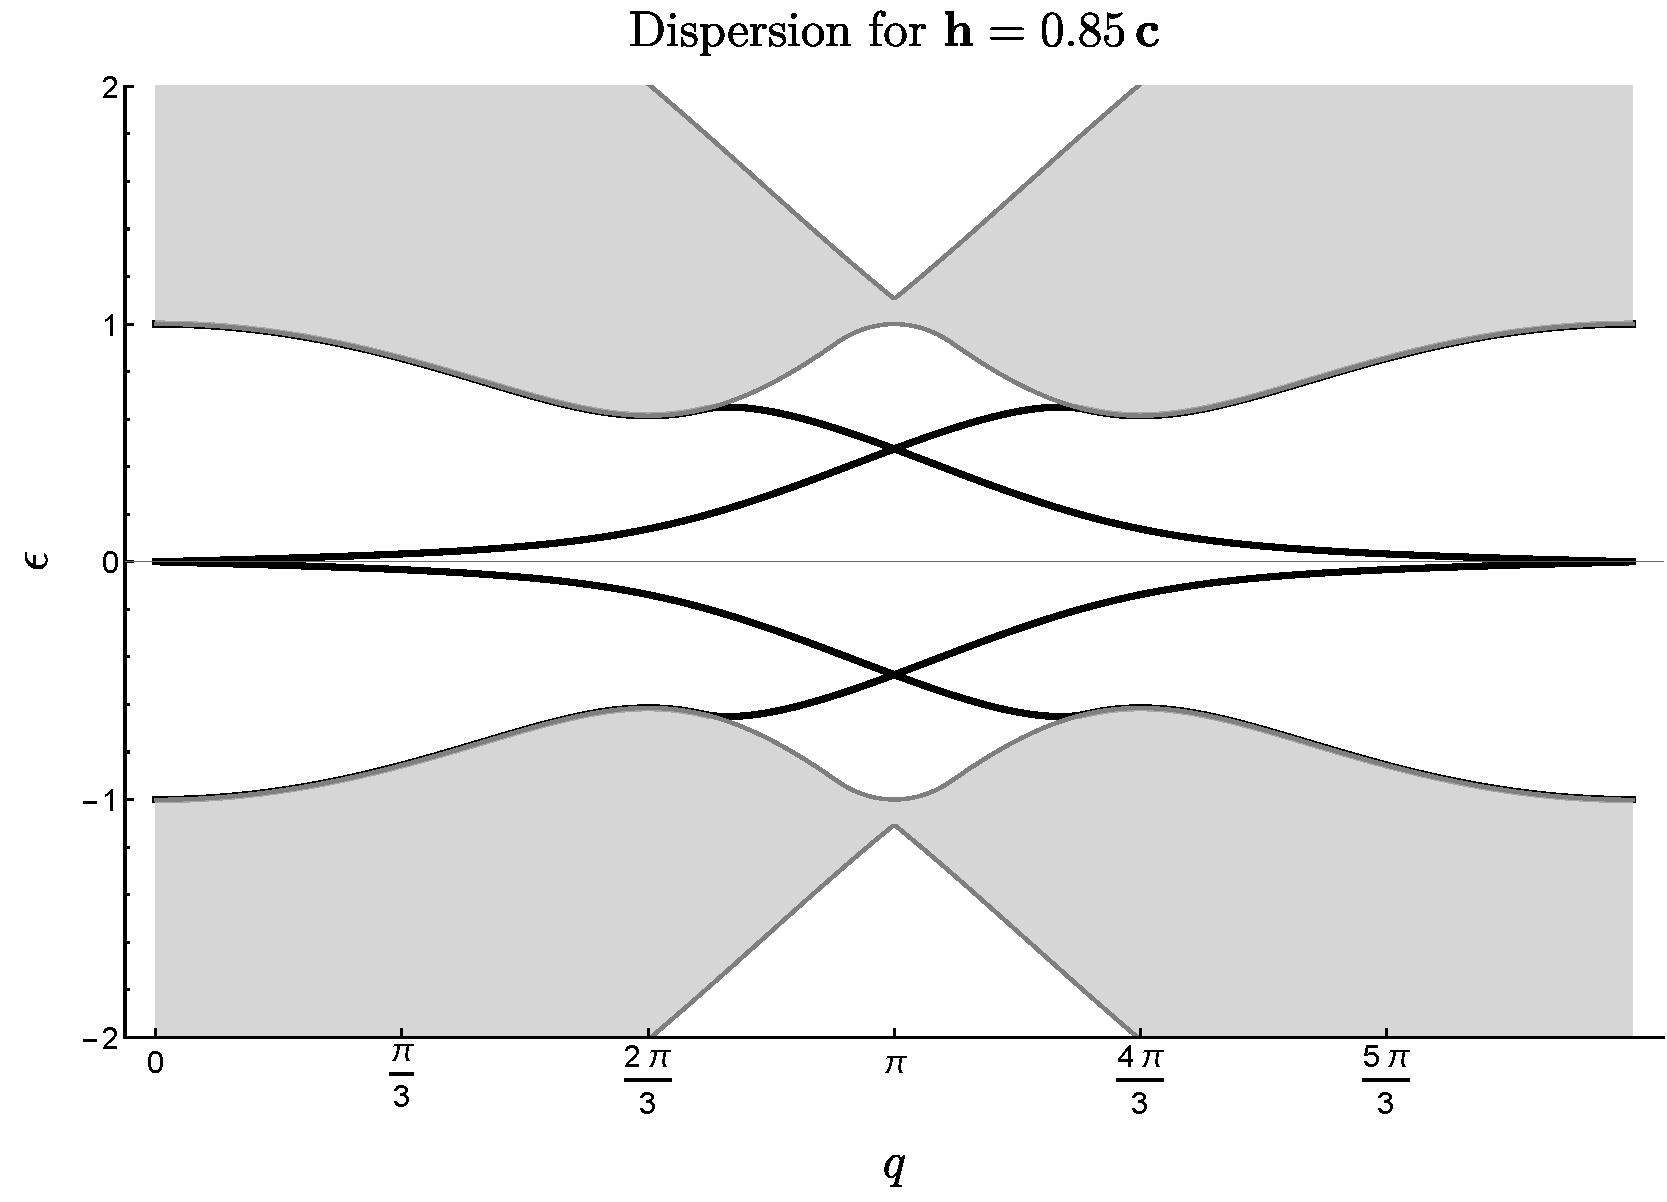
\includegraphics[width = 0.9 \textwidth]{images/CH3/disp_c.pdf}   \end{minipage}    \caption{(Left) Magnetic field in the $\bf{a}$ direction with modulus $0.85 \, J$. The bulk is gapped and the edge is gapless.  (Right) Magnetic field in the $\bf{b}$ direction with modulus $0.85 \, J$. The gap in the bulk is zero.     }  \label{fig:3-disp-ab}   \end{figure}
  

  


